\mfpicnumber{1}

\opengraphsfile{IntroExpLogs}

\setcounter{footnote}{0}

\label{IntroExpLogs}

Of all of the  functions we study in this text, exponential and logarithmic functions are possibly the ones which impact everyday life the most.\footnote{Take a class in Differential Equations and you'll see why.} This section will introduce us to these functions while the rest of the chapter will more thoroughly explore their properties.  Up to this point, we have dealt with functions which involve terms like $x^2$ or $x^{2/3}$, in other words, terms of the form  $x^{p}$ where the base of the term, $x$, varies but the exponent of each term, $p$, remains constant.  In this chapter, we study functions of the form $f(x) = b^{x}$ where the base $b$ is a constant and the exponent $x$ is the variable.  We start our exploration of these functions with $f(x) = 2^{x}$. (Apparently this is a tradition.  Every College Algebra book we have ever read starts with $f(x) = 2^{x}$.) We make a table of values, plot the points and connect them in a pleasing fashion.

\hspace{1in} \begin{tabular}{m{2.7in}m{3in}}

\setlength{\extrarowheight}{4pt}
\[ \begin{array}{|r||r|r|}  

\hline

 x & f(x) & (x,f(x)) \\ \hline
-3  & 2^{-3} = \frac{1}{8} & \left(-3, \frac{1}{8} \right) \\ [2pt] \hline
-2  & 2^{-2} = \frac{1}{4} &  \left(-2, \frac{1}{4} \right) \\ [2pt] \hline
-1 & 2^{-1} &  \left(-1, \frac{1}{2} \right) \\ [2pt]  \hline
0  & 2^{0} = 1 & ( 0 ,1) \\  \hline
1 & 2^{1} = 2 & ( 1, 2) \\  \hline
2  & 2^{2} = 4 & (2,4) \\  \hline
3  & 2^{3}=8 & (3, 8) \\  \hline
\end{array} \] 
\setlength{\extrarowheight}{2pt}

&

\begin{mfpic}[13]{-4}{4}{-1}{9}
\point[2pt]{(-3,0.125), (-2,0.25), (-1,0.5), (0,1), (1,2), (2,4), (3,8)}
\axes
\tlabel[cc](4,-0.5){\scriptsize $x$}
\tlabel[cc](0.5,9){\scriptsize $y$}
\tcaption{\scriptsize $y = f(x) = 2^{x}$}
\xmarks{-3,-2,-1,1,2,3}
\ymarks{1,2,3,4,5,6,7,8}
\tlpointsep{4pt}
\axislabels {x}{{\tiny $-3 \hspace{7pt}$} -3, {\tiny $-2 \hspace{7pt}$} -2, {\tiny $-1 \hspace{7pt}$} -1, {\tiny $1$} 1, {\tiny $2$} 2, {\tiny $3$} 3}
\axislabels {y}{{\tiny $1$} 1, {\tiny $2$} 2, {\tiny $3$} 3, {\tiny $4$} 4, {\tiny $5$} 5, {\tiny $6$} 6, {\tiny $7$} 7, {\tiny $8$} 8}
\arrow \reverse \arrow \function{-3.5, 3.1, 0.1}{2**x}
\end{mfpic} \\

\end{tabular}

A few remarks about the graph of $f(x) = 2^{x}$ which we have constructed are in order.  As $x \rightarrow -\infty$ and attains values like $x = -100$ or $x=-1000$, the function $f(x) = 2^{x}$ takes on values like $f(-100) = 2^{-100} = \frac{1}{2^{100}}$ or $f(-1000) = 2^{-1000} = \frac{1}{2^{1000}}$.  In other words, as $x \rightarrow -\infty$, \[2^{x} \approx \frac{1}{\mbox{very big $(+)$}}  \approx \mbox{very small $(+)$}\]  So as $x \rightarrow -\infty$, $2^{x} \rightarrow 0^{+}$.  This is represented graphically using the $x$-axis (the line $y = 0$) as a horizontal asymptote.  On the flip side, as $x \rightarrow \infty$, we find $f(100) = 2^{100}$, $f(1000) = 2^{1000}$, and so on, thus $2^{x} \rightarrow \infty$. As a result, our graph suggests the range of $f$ is $(0,\infty)$.  The graph of $f$ passes the Horizontal Line Test which means $f$ is one-to-one and hence invertible.  We also note that when we `connected the dots in a pleasing fashion', we have made the implicit assumption that $f(x) = 2^{x}$ is continuous\footnote{Recall that this means there are no holes or other kinds of breaks in the graph.} and has a domain of all real numbers.  In particular, we have suggested that things like $2^{\sqrt{3}}$ exist as real numbers.  We should take a moment to discuss what something like $2^{\sqrt{3}}$ might mean, and refer the interested reader to a solid course in Calculus for a more rigorous explanation.  The number $\sqrt{3} = 1.73205 \ldots$ is an irrational number\footnote{You can actually prove this by considering the polynomial $p(x) = x^2-3$ and showing it has no rational zeros by applying Theorem \ref{RZT}.} and as such, its decimal representation neither repeats nor terminates.  We can, however, approximate $\sqrt{3}$ by terminating decimals, and it stands to reason\footnote{This is where Calculus and continuity come into play.} we can use these to approximate $2^{\sqrt{3}}$.  For example, if we approximate $\sqrt{3}$ by $1.73$, we can approximate $2^{\sqrt{3}} \approx 2^{1.73} = 2^{\frac{173}{100}} = \sqrt[100]{2^{173}}$. It is not, by any means, a pleasant number, but it is at least a number that we understand in terms of powers and roots.  It also stands to reason that better and better approximations of $\sqrt{3}$ yield better and better approximations of $2^{\sqrt{3}}$, so the value of $2^{\sqrt{3}}$ should be the result of this sequence of approximations.\footnote{Want more information?  Look up ``convergent sequences'' on the Internet.}
  
\smallskip

Suppose we wish to study the family of functions $f(x) = b^{x}$.  Which bases $b$ make sense to study?  We find that we run into difficulty if $b < 0$.  For example, if $b = -2$, then the function $f(x) = (-2)^{x}$ has trouble, for instance, at $x = \frac{1}{2}$ since $(-2)^{1/2} = \sqrt{-2}$ is not a real number. In general, if $x$ is any rational number with an even denominator, then $(-2)^{x}$ is not defined, so we must restrict our attention to bases $b \geq 0$.  What about $b = 0$?  The function $f(x) = 0^{x}$ is undefined for $x \leq 0$ because we cannot divide by $0$ and $0^{0}$ is an indeterminant form.  For $x > 0$, $0^{x} = 0$ so the function  $f(x) = 0^{x}$ is the same as the function $f(x) = 0$, $x > 0$. \phantomsection \label{indeterminantformtwo} We know everything we can possibly know about this function, so we exclude it from our investigations.  The only other base we exclude is $b=1$, since the function $f(x) = 1^{x} = 1$ is, once again, a function we have already studied.  We are now ready for our definition of exponential functions.

\smallskip


\colorbox{ResultColor}{\bbm

\begin{defn} \label{expfcndefn}  A function of the form $f(x) = b^{x}$ where $b$ is a fixed real number, $b > 0$, $b \neq 1$ is called a \index{function ! exponential} \index{exponential function ! definition of} \textbf{base \emph{b} exponential function}.

\end{defn}


\ebm}
\smallskip

We leave it to the reader to verify\footnote{Meaning, graph some more examples on your own.} that if $b > 1$, then the exponential function $f(x) = b^{x}$ will share the same basic shape and characteristics as $f(x) = 2^{x}$.  What if $0 < b < 1$?  Consider $g(x) = \left(\frac{1}{2}\right)^{x}$.  We could certainly build a table of values and connect the points, or we could take a step back and note that $g(x) = \left(\frac{1}{2}\right)^{x} = \left(2^{-1}\right)^{x} = 2^{-x} = f(-x)$, where $f(x) = 2^{x}$.  Thinking back to Section \ref{Transformations}, the graph of $f(-x)$ is obtained from the graph of $f(x)$ by reflecting it across the $y$-axis. We get

\[\begin{array}{ccc}

\begin{mfpic}[10]{-4}{4}{-1}{9}
\point[2pt]{(-3,0.125), (-2,0.25), (-1,0.5), (0,1), (1,2), (2,4), (3,8)}
\axes
\tlabel[cc](4,-0.5){\scriptsize $x$}
\tlabel[cc](0.5,9){\scriptsize $y$}
\tcaption{\scriptsize $y = f(x) = 2^{x}$}
\xmarks{-3,-2,-1,1,2,3}
\ymarks{1,2,3,4,5,6,7,8}
\tlpointsep{4pt}
\axislabels {x}{{\tiny $-3 \hspace{7pt}$} -3, {\tiny $-2 \hspace{7pt}$} -2, {\tiny $-1 \hspace{7pt}$} -1, {\tiny $1$} 1, {\tiny $2$} 2, {\tiny $3$} 3}
\axislabels {y}{{\tiny $1$} 1, {\tiny $2$} 2, {\tiny $3$} 3, {\tiny $4$} 4, {\tiny $5$} 5, {\tiny $6$} 6, {\tiny $7$} 7, {\tiny $8$} 8}
\arrow \reverse \arrow \function{-3.5, 3.1, 0.1}{2**x}
\end{mfpic}

&

\stackrel{\stackrel{\mbox{\scriptsize reflect across $y$-axis}}{\xrightarrow{\hspace{1in}}}}{\mbox{ \scriptsize multiply each $x$-coordinate by $-1$}} 

&

\begin{mfpic}[10]{-4}{4}{-1}{9}
\point[2pt]{(3,0.125), (2,0.25), (1,0.5), (0,1), (-1,2), (-2,4), (-3,8)}
\axes
\tlabel[cc](4,-0.5){\scriptsize $x$}
\tlabel[cc](0.5,9){\scriptsize $y$}
\tcaption{\scriptsize $y = g(x) = 2^{-x} = \left(\frac{1}{2}\right)^{x}$}
\xmarks{-3,-2,-1,1,2,3}
\ymarks{1,2,3,4,5,6,7,8}
\tlpointsep{4pt}
\axislabels {x}{{\tiny $-3 \hspace{7pt}$} -3, {\tiny $-2 \hspace{7pt}$} -2, {\tiny $-1 \hspace{7pt}$} -1, {\tiny $1$} 1, {\tiny $2$} 2, {\tiny $3$} 3}
\axislabels {y}{{\tiny $1$} 1, {\tiny $2$} 2, {\tiny $3$} 3, {\tiny $4$} 4, {\tiny $5$} 5, {\tiny $6$} 6, {\tiny $7$} 7, {\tiny $8$} 8}
\arrow \reverse \arrow \function{-3.1, 3.5, 0.1}{(0.5)**x}
\end{mfpic} \\

\end{array}\]

We see that the domain and range of $g$ match that of $f$, namely $(-\infty, \infty)$ and $(0,\infty)$, respectively. Like $f$, $g$ is also one-to-one.  Whereas $f$ is always increasing, $g$ is always decreasing.  As a result, as $x \rightarrow -\infty$, $g(x) \rightarrow \infty$, and on the flip side, as $x \rightarrow \infty$, $g(x) \rightarrow 0^{+}$.  It shouldn't be too surprising that for all choices of the base $0 < b < 1$, the graph of $y=b^{x}$ behaves similarly to the graph of $g$.  We summarize the basic properties of exponential functions in the following theorem.\footnote{The proof of which, like many things discussed in the text, requires Calculus.}

\smallskip

\colorbox{ResultColor}{\bbm

\begin{thm} \label{expfcnprops} \textbf{Properties of Exponential Functions:} Suppose $f(x) = b^{x}$. \index{exponential function ! graphical properties of}

\begin{itemize}

\item  The domain of $f$ is $(-\infty, \infty)$ and the range of $f$ is $(0, \infty)$.

\item  $(0,1)$ is on the graph of $f$ and $y=0$ is a horizontal asymptote to the graph of $f$.

\item  $f$ is one-to-one, continuous and smooth\footnote{Recall that this means the graph of $f$ has no sharp turns or corners.}

\end{itemize}

\begin{tabular}{m{2.5in}m{2.5in}}

\begin{itemize}

\item  If $b > 1$:

\begin{itemize}

\item  $f$ is always increasing

\item  As $x \rightarrow -\infty$, $f(x) \rightarrow 0^{+}$

\item  As $x \rightarrow \infty$, $f(x) \rightarrow \infty$

\item  The graph of $f$ resembles:

\begin{center}

\begin{mfpic}[10]{-3}{3}{-1}{5}

\axes

\ymarks{1}

\arrow \reverse \arrow \function{-2.3,2.3,0.1}{2**x}

\tcaption{\scriptsize $y = b^{x}$, $b > 1$}

\end{mfpic}

\end{center}

\end{itemize}

\end{itemize}

&
\begin{itemize}

\item  If $0<b<1$:

\begin{itemize}

\item  $f$ is always decreasing

\item  As $x \rightarrow -\infty$, $f(x) \rightarrow \infty$

\item  As $x \rightarrow \infty$, $f(x) \rightarrow 0^{+}$

\item  The graph of $f$ resembles:

\begin{center}

\begin{mfpic}[10]{-3}{3}{-1}{5}

\axes

\ymarks{1}

\arrow \reverse \arrow \function{-2.3,2.3,0.1}{(0.5)**x}

\tcaption{\scriptsize $y = b^{x}$, $0 < b < 1$}

\end{mfpic}


\end{center}

\end{itemize}

\end{itemize} \\

\end{tabular}

\end{thm}

\ebm}

\smallskip

Of all of the bases for exponential functions, two occur the most often in scientific circles.  The first, base $10$, is often called the \index{exponential function ! common base} \index{common base} \textbf{common base}.  The second base is an irrational number, $e \approx 2.718$, called the \index{natural base} \index{exponential function ! natural base} \textbf{natural base}.  We will more formally discuss the origins of this number in Section \ref{ExpLogApplications}.  For now, it is enough to know that since $e > 1$, $f(x) = e^{x}$ is an increasing exponential function.  The following examples give us an idea how these functions are used in the wild.

\begin{ex}  \label{cardepreciationex} The value of a car can be modeled by $V(x) = 25\left(\frac{4}{5}\right)^{x}$, where $x \geq 0$ is age of the car in years and $V(x)$ is the value in thousands of dollars. \index{depreciation}

\begin{enumerate}

\item  Find and interpret $V(0)$.

\item  Sketch the graph of $y=V(x)$ using transformations.

\item  Find and interpret the horizontal asymptote of the graph you found in 2.

\end{enumerate}

{\bf Solution.}

\begin{enumerate}

\item  To find $V(0)$, we replace $x$ with $0$ to obtain $V(0) = 25\left(\frac{4}{5}\right)^{0} = 25$.  Since $x$ represents the age of the car in years, $x=0$ corresponds to the car being brand new.  Since $V(x)$ is measured in thousands of dollars, $V(0)=25$ corresponds to a value of $\$ 25,\!000$.  Putting it all together, we interpret $V(0)=25$ to mean the purchase price of the car was $\$25,\!000$.

\item  To graph $y=25\left(\frac{4}{5}\right)^{x}$,  we start with the basic exponential function $f(x)=\left(\frac{4}{5}\right)^{x}$.  Since the base $b = \frac{4}{5}$ is between $0$ and $1$, the graph of $y=f(x)$ is decreasing.  We plot the $y$-intercept $(0,1)$ and two other points, $\left(-1, \frac{5}{4}\right)$ and $\left(1, \frac{4}{5}\right)$, and label the horizontal asymptote $y=0$.  To obtain $V(x) = 25\left(\frac{4}{5}\right)^{x}$, $x \geq 0$, we multiply the output from $f$ by $25$, in other words, $V(x) = 25 f(x)$. In accordance with Theorem \ref{vscalings}, this results in a vertical stretch by a factor of $25$.  We multiply all of the $y$ values in the graph by $25$ (including the $y$ value of the horizontal asymptote) and obtain the points $\left(-1,\frac{125}{4}\right)$, $(0,25)$ and $(1,20)$. The horizontal asymptote remains $y=0$. Finally, we restrict the domain to $[0,\infty)$ to fit with the applied domain given to us.  We have the result below.

\[\begin{array}{ccc}

\begin{mfpic}[10][20]{-4}{4}{-1}{3}
\point[2pt]{(0,1),(1,0.8), (-1,1.25)}
\axes
\tlabel[cc](1,1.25){\tiny $(0,1)$}
\tlabel[cc](0,-1.5){\tiny H.A. $y=0$}
\tlabel[cc](4,-0.5){\tiny $x$}
\tlabel[cc](0.5,3){\tiny $y$}
\tcaption{\scriptsize $y = f(x)=\left(\frac{4}{5}\right)^{x}$}
\ymarks{1,2}
\xmarks{-3,-2,-1,1,2,3}
\tlpointsep{4pt}
\axislabels {x}{{\tiny $-3 \hspace{7pt}$} -3, {\tiny $-2 \hspace{7pt}$} -2, {\tiny $-1 \hspace{7pt}$} -1, {\tiny $1$} 1, {\tiny $2$} 2, {\tiny $3$} 3}
\axislabels {y}{{\tiny $2$} 2}
\arrow \reverse \arrow \function{-4, 4, 0.1}{(0.8)**x}
\end{mfpic}

&

\stackrel{\stackrel{\mbox{\scriptsize vertical scale by a factor of $25$ }}{\xrightarrow{\hspace{1.75in}}}}{\mbox{ \scriptsize multiply each $y$-coordinate by $25$}} 

&

\begin{mfpic}[10]{-1}{7}{-1}{7}
\point[2pt]{(0,5),(1,4)}
\axes
\tlabel[cc](-1.5,5){\tiny $(0,25)$}
\tlabel[cc](4,-1.5){\tiny H.A. $y=0$}
\tlabel[cc](7,-0.5){\tiny $x$}
\tlabel[cc](0.5,7){\tiny $y$}
\tcaption{\scriptsize $y = V(x)=25 f(x)$, $x \geq 0$}
\ymarks{1,2,3,4,5,6}
\xmarks{1,2,3,4,5,6}
\tlpointsep{4pt}
\axislabels {x}{{\tiny $1$} 1, {\tiny $2$} 2, {\tiny $3$} 3, {\tiny $4$} 4, {\tiny $5$} 5, {\tiny $6$} 6}
\axislabels {y}{{\tiny $5$} 1, {\tiny $10$} 2, {\tiny $15$} 3, {\tiny $20$} 4, {\tiny $30$} 6}
\arrow \function{0, 7, 0.1}{5*((0.8)**x)}
\end{mfpic} \\

\end{array}\]

\item  We see from the graph of $V$ that its horizontal asymptote is $y=0$.  (We leave it to reader to verify this analytically by thinking about what happens as we take larger and larger powers of $\frac{4}{5}$.)  This means as the car gets older, its value diminishes to $0$.  \qed
 
\end{enumerate}

\end{ex}

The function in the previous example is often called a `decay curve'.  Increasing exponential functions are used to model `growth curves' and we shall see several different examples of those in Section \ref{ExpLogApplications}.  For now, we present another common decay curve which will serve as the basis for further study of exponential functions.  Although it may look more complicated than the previous example, it is actually just a basic exponential function which has been modified by a few transformations from Section \ref{Transformations}.

\begin{ex}  \label{exptempex} According to \href{http://en.wikipedia.org/wiki/Heat_transfer#Newton.27s_law_of_cooling}{\underline{Newton's Law of Cooling}}\footnote{We will discuss this in greater detail in Section \ref{ExpLogApplications}.} the temperature of coffee $T$ (in degrees Fahrenheit) $t$ minutes after it is served can be modeled by $T(t) = 70 + 90 e^{-0.1 t}$. \index{Newton's Law of Cooling}

\begin{enumerate}

\item  Find and interpret $T(0)$.

\item  Sketch the graph of $y = T(t)$ using transformations.

\item  Find and interpret the horizontal asymptote of the graph.

\end{enumerate}

{\bf Solution.}

\begin{enumerate}

\item  To find $T(0)$, we replace every occurrence of the independent variable $t$ with $0$ to obtain  $T(0) =70 + 90 e^{-0.1 (0)} = 160$.  This means that the coffee was served at $160^{\circ}\mbox{F}$.

\item  To graph $y = T(t)$ using transformations, we start with the basic function, $f(t)=e^{t}$.  As we have already remarked, $e \approx 2.718 > 1$ so the graph of $f$ is an increasing exponential with $y$-intercept $(0,1)$ and horizontal asymptote $y = 0$.  The points $\left(-1, e^{-1}\right) \approx (-1,0.37)$ and $(1,e) \approx (1,2.72)$ are also on the graph.  Since the formula $T(t)$ looks rather complicated, we rewrite $T(t)$ in the form presented in Theorem  \ref{transformationsthm} and use that result to track the changes to our three points and the horizontal asymptote.  We have \[T(t) = 70 + 90e^{-0.1t} = 90e^{-0.1t}+70 = 90 f(-0.1t)+70\]  Multiplication of the input to $f$, $t$, by $-0.1$ results in a horizontal expansion by a factor of $10$ as well as a reflection about the $y$-axis.  We divide each of the $x$ values of our points by $-0.1$ (which amounts to multiplying them by $-10$) to obtain $\left(10,e^{-1}\right)$, $(0,1)$, and $\left(-10, e\right)$.  Since none of these changes affected the $y$ values, the horizontal asymptote remains $y = 0$.  Next, we see that the output from $f$ is being multiplied by $90$.  This results in a vertical stretch by a factor of $90$.  We multiply the $y$-coordinates by $90$ to obtain $\left(10,90e^{-1}\right)$, $(0,90)$, and $\left(-10, 90e\right)$. We also multiply the $y$ value of the horizontal asymptote $y=0$ by $90$, and it remains $y=0$.  Finally, we add $70$ to all of the $y$-coordinates, which shifts the graph upwards to obtain $\left(10,90e^{-1} + 70\right) \approx (10, 103.11)$, $(0,160)$, and $\left(-10, 90e+ 70\right) \approx (-10,314.64)$.  Adding $70$ to the horizontal asymptote shifts it upwards as well to $y=70$.  We connect these three points using the same shape in the same direction as in the graph of $f$ and, last but not least, we restrict the domain to match the applied domain $[0, \infty)$.  The result is below.  


\[\begin{array}{ccc}

\begin{mfpic}[10]{-4}{4}{-1}{8}
\point[2pt]{(0,1),(1,2.718), (-1,0.368)}
\axes
\tlabel[cc](-1,1){\tiny $(0,1)$}
\tlabel[cc](0,-1.5){\tiny H.A. $y=0$}
\tlabel[cc](4,-0.5){\tiny $t$}
\tlabel[cc](0.5,8){\tiny $y$}
\tcaption{\scriptsize $y = f(t)=e^{t}$}
\ymarks{1,2,3,4,5,6,7}
\xmarks{-3,-2,-1,1,2,3}
\tlpointsep{4pt}
\axislabels {x}{{\tiny $-3 \hspace{7pt}$} -3, {\tiny $-2 \hspace{7pt}$} -2, {\tiny $-1 \hspace{7pt}$} -1, {\tiny $1$} 1, {\tiny $2$} 2, {\tiny $3$} 3}
\axislabels {y}{{\tiny $2$} 2,{\tiny $3$} 3,{\tiny $4$} 4,{\tiny $5$} 5,{\tiny $6$} 6,{\tiny $7$} 7}
\arrow \reverse \arrow \function{-3, 2, 0.1}{exp(x)}
\end{mfpic}

&
\xrightarrow{\hspace{1in}}
&

\begin{mfpic}[10]{-1}{11}{-1}{10}
\point[2pt]{(0,8),(5,5.15)}
\dashed \polyline{(-1,3.5),(11,3.5)}
\axes
\tlabel[cc](9,2.5){\tiny H.A. $y=70$}
\tlabel[cc](11,-0.5){\tiny $t$}
\tlabel[cc](0.5,10){\tiny $y$}
\tcaption{\scriptsize $y = T(t)$}
\ymarks{1,2,3,4,5,6,7,8,9}
\xmarks{1,2,3,4,5,6,7,8,9,10}
\tlpointsep{4pt}
\axislabels {x}{{\tiny $2$} 1, {\tiny $4$} 2, {\tiny $6$} 3, {\tiny $8$} 4,{\tiny $10$} 5, {\tiny $12$} 6, {\tiny $14$} 7, {\tiny $16$} 8, {\tiny $18$} 9, {\tiny $20$} 10}
\axislabels {y}{{\tiny $20$} 1, {\tiny $40$} 2, {\tiny $60$} 3,{\tiny $80$} 4, {\tiny $100$} 5, {\tiny $120$} 6,{\tiny $140$} 7, {\tiny $160$} 8, {\tiny $180$} 9}
\arrow \function{0, 10, 0.1}{(90*exp(0-0.2*x)+70)/20}
\end{mfpic} \\

\end{array}\]

\item  From the graph, we see that the horizontal asymptote is $y = 70$. It is worth a moment or two of our time to see how this happens analytically and to review some of the `number sense' developed in Chapter \ref{Rationals}.  As $t \rightarrow \infty$, We get $T(t) = 70+90e^{-0.1t} \approx 70 +90e^{\mbox{\tiny very big $(-)$}}$.  Since $e > 1$, \[e^{\mbox{\tiny very big $(-)$}} = \frac{1}{e^{\mbox{\tiny very big $(+)$}}} \approx \frac{1}{\mbox{\tiny very big $(+)$}} \approx \mbox{very small $(+)$}\]  The larger $t$ becomes, the smaller $e^{-0.1t}$ becomes, so the term $90 e^{-0.1t} \approx \mbox{very small $(+)$}$.  Hence, $T(t) \approx 70 + \mbox{very small $(+)$}$ which means the graph is approaching the horizontal line $y=70$ from above.  This means that as time goes by, the temperature of the coffee is cooling to $70^{\circ}\mbox{F}$, presumably room temperature.  \qed

\end{enumerate}

\end{ex}

As we have already remarked, the graphs of $f(x) = b^{x}$ all pass the Horizontal Line Test.  Thus the exponential functions are invertible.   We now turn our attention to these inverses, the logarithmic functions, which are called `logs' for short.

\smallskip

\colorbox{ResultColor}{\bbm

\begin{defn} \label{logfcndefn} The inverse of the exponential function $f(x) = b^{x}$ is called the \index{function ! logarithmic} \textbf{base \boldmath $b$ logarithm function}, and is denoted  $f^{-1}(x) = \log_{b}(x)$  The expression $\log_{b}(x)$ is read `log base $b$ of $x$.' \index{logarithm ! general, ``base $b$''}

\end{defn}

\ebm}
\smallskip

We have special notations for the common base, $b=10$, and the natural base, $b=e$.


\smallskip

\colorbox{ResultColor}{\bbm

\begin{defn} The \index{logarithm ! common} \textbf{common logarithm} of a real number $x$ is $\log_{10}(x)$ and is usually written $\log(x)$.   The \index{logarithm ! natural} \textbf{natural logarithm} of a real number $x$ is $\log_{e}(x)$ and is usually written $\ln(x)$. \index{common logarithm} \index{natural logarithm}

\end{defn}

\ebm}
\smallskip

Since logs are defined as the inverses of exponential functions, we can use Theorems \ref{inversefunctionprops} and \ref{inverseuniquegraph} to tell us about logarithmic functions.  For example, we know that the domain of a log function is the range of an exponential function, namely $(0, \infty)$, and that the range of a log function is the domain of an exponential function, namely $(-\infty, \infty)$.   Since we know the basic shapes of $y = f(x) = b^{x}$ for the different cases of $b$, we can obtain the graph of $y = f^{-1}(x) = \log_{b}(x)$ by reflecting the graph of $f$ across the line $y=x$ as shown below.  The $y$-intercept $(0,1)$ on the graph of $f$  corresponds to an $x$-intercept of $(1,0)$ on the graph of $f^{-1}$.  The horizontal asymptotes $y=0$ on the graphs of the exponential functions become vertical asymptotes $x=0$ on the log graphs.  

\[ \begin{array}{cc}

\begin{mfpic}[10]{-3}{5}{-3}{5}
\axes
\xmarks{1}
\ymarks{1}
\arrow \reverse \arrow \function{-2.3, 2.3, 0.1}{2**x}
\dashed \polyline{(-1,-1), (5,5)}
\tlabel[cc](3,-4){\scriptsize $y =b^{x}$, $b > 1$}
\tlabel[cc](3,-5){\scriptsize \mbox{\boldmath $y = \log_{b}(x)$}, $b > 1$}
\penwd{1.5pt}
\arrow \reverse \arrow \parafcn{-2.3,2.3,0.1}{(2^t,t)}
\end{mfpic}

& 

\hspace{1.5in}

\begin{mfpic}[10]{-3}{5}{-3}{5}
\axes
\xmarks{1}
\ymarks{1}
\arrow \reverse \arrow \function{-2.3, 2.3, 0.1}{(0.5)**x}
\dashed \polyline{(-1,-1), (5,5)}
\tlabel[cc](3,-4){\scriptsize $y =b^{x}$, $0 < b < 1$}
\tlabel[cc](3,-5){\scriptsize \mbox{\boldmath $y = \log_{b}(x)$}, $0 < b < 1$}
\penwd{1.5pt}
\arrow \reverse \arrow \parafcn{-2.3,2.3,0.1}{(2^t,-t)}
\end{mfpic}

\end{array}\]

On a procedural level, logs undo the exponentials.  Consider the function $f(x) = 2^{x}$.  When we evaluate $f(3) = 2^{3} = 8$, the input $3$ becomes the exponent on the base $2$ to produce the real number $8$.  The function $f^{-1}(x) = \log_{2}(x)$ then takes the number $8$ as its input and returns the exponent $3$ as its output.  In symbols, $\log_{2}(8) = 3$. More generally, $\log_{2}(x)$ is the exponent you put on $2$ to get $x$.  Thus, $\log_{2}(16) = 4$, because $2^{4} = 16$.  The following theorem summarizes the basic properties of logarithmic functions, all of which come from the fact that they are inverses of exponential functions. 
\smallskip

\colorbox{ResultColor}{\bbm

\begin{thm} \label{logfcnprops} \textbf{Properties of Logarithmic Functions:} Suppose $f(x) = \log_{b}(x)$. \index{logarithm ! graphical properties of}

\begin{itemize}

\item  The domain of $f$ is $(0, \infty)$ and the range of $f$ is $(-\infty, \infty)$.

\item  $(1,0)$ is on the graph of $f$ and $x=0$ is a vertical asymptote of the graph of $f$.

\item  $f$ is one-to-one, continuous and smooth

\item  $b^{a} = c$ if and only if $\log_{b}(c) = a$.  That is, $\log_{b}(c)$ is the exponent you put on $b$ to obtain $c$.

\item  $\log_{b} \left(b^{x}\right) = x$ for all $x$ and $b^{\log_{b}(x)} = x$ for all $x > 0$

\end{itemize}

\begin{tabular}{m{2.5in}m{2.5in}}

\begin{itemize}

\item  If $b > 1$:

\begin{itemize}

\item  $f$ is always increasing

\item  As $x \rightarrow 0^{+}$, $f(x) \rightarrow -\infty$

\item  As $x \rightarrow \infty$, $f(x) \rightarrow \infty$

\item  The graph of $f$ resembles:

\begin{center}

\begin{mfpic}[10]{-1}{5}{-3}{3}
\axes
\xmarks{1}
\arrow \reverse \arrow \parafcn{-2.3,2.3,0.1}{(2^t,t)}
\tlabel[cc](3,-4){\scriptsize $y = \log_{b}(x)$, $b > 1$}
\end{mfpic}

\end{center}

\end{itemize}

\end{itemize}

&
\begin{itemize}

\item  If $0<b<1$:

\begin{itemize}

\item  $f$ is always decreasing

\item  As $x \rightarrow 0^{+}$, $f(x) \rightarrow \infty$

\item  As $x \rightarrow \infty$, $f(x) \rightarrow -\infty$

\item  The graph of $f$ resembles:

\begin{center}

\begin{mfpic}[10]{-1}{5}{-3}{3}
\axes
\xmarks{1}
\arrow \reverse \arrow \parafcn{-2.3,2.3,0.1}{(2^t,-t)}
\tlabel[cc](3,-4){\scriptsize $y = \log_{b}(x)$, $0 < b < 1$}
\end{mfpic}

\end{center}
\end{itemize}

\end{itemize} \\

\end{tabular}

\end{thm}

\ebm}

\smallskip

As we have mentioned, Theorem \ref{logfcnprops} is a consequence of Theorems \ref{inversefunctionprops} and \ref{inverseuniquegraph}.  However, it is worth the reader's time to understand Theorem \ref{logfcnprops} from an exponential perspective.  For instance, we know that the domain of $g(x) = \log_{2}(x)$ is $(0,\infty)$.  Why?  Because the range of $f(x) = 2^{x}$ is $(0,\infty)$.  In a way, this says everything, but at the same time, it doesn't. For example, if we try to find $\log_{2}(-1)$, we are trying to find the exponent we put on $2$ to give us $-1$.  In other words, we are looking for $x$ that satisfies $2^{x} = -1$.  There is no such real number, since all powers of $2$ are positive.  While what we have said is exactly the same thing as saying `the domain of $g(x) = \log_{2}(x)$ is $(0,\infty)$ because the range of $f(x) = 2^{x}$ is $(0,\infty)$', we feel it is in a student's best interest to understand the statements in Theorem \ref{logfcnprops} at this level instead of just merely memorizing the facts.

\begin{ex}  Simplify the following.

\begin{multicols}{4}
\begin{enumerate}

\item  $\log_{3}(81)$

\item  $\log_{2}\left(\dfrac{1}{8}\right)$

\item  $\log_{\sqrt{5}}(25)$

\item  $\ln\left(\sqrt[3]{e^2}\right)$

\setcounter{HW}{\value{enumi}}
\end{enumerate}
\end{multicols}

\begin{multicols}{4}
\begin{enumerate}
\setcounter{enumi}{\value{HW}}

\item  $\log(0.001)$

\item  $2^{\log_{2}(8)}$

\item  $117^{-\log_{117}(6)}$

\end{enumerate}
\end{multicols}


{\bf Solution.}

\begin{enumerate}

\item The number $\log_{3}(81)$ is the exponent we put on $3$ to get $81$.  As such, we want to write $81$ as a power of $3$.  We find $81 = 3^{4}$, so that $\log_{3}(81)=4$.

\item To find $\log_{2}\left(\frac{1}{8}\right)$, we need rewrite $\frac{1}{8}$ as a power of $2$.  We find $\frac{1}{8} = \frac{1}{2^{3}} = 2^{-3}$, so $\log_{2}\left(\frac{1}{8}\right) = -3$.

\item To determine $\log_{\sqrt{5}}(25)$, we need to express $25$ as a power of $\sqrt{5}$.  We know $25 = 5^2$, and $5 = \left(\sqrt{5}\right)^2$, so we have $25 = \left(\left(\sqrt{5}\right)^2\right)^2 = \left(\sqrt{5}\right)^4$.  We get $\log_{\sqrt{5}}(25) = 4$.

\item  First, recall that the notation  $\ln\left(\sqrt[3]{e^2}\right)$ means $\log_{e}\left(\sqrt[3]{e^2}\right)$, so we are looking for the exponent to put on $e$ to obtain $\sqrt[3]{e^2}$.  Rewriting $\sqrt[3]{e^2} = e^{2/3}$, we find  $\ln\left(\sqrt[3]{e^2}\right) =  \ln\left(e^{2/3}\right) = \frac{2}{3}$.

\item  Rewriting $\log(0.001)$ as $\log_{10} (0.001)$, we see that we need to write $0.001$ as a power of $10$.  We have $0.001 = \frac{1}{1000} = \frac{1}{10^3} = 10^{-3}$.  Hence, $\log(0.001) = \log\left(10^{-3}\right) = -3$.

\item  We can use Theorem \ref{logfcnprops} directly to simplify  $2^{\log_{2}(8)} = 8$. We can also understand this problem by first finding $\log_{2}(8)$.  By definition, $\log_{2}(8)$ is the exponent we put on $2$ to get $8$.  Since $8 = 2^3$, we have $\log_{2}(8) = 3$.  We now substitute to find $2^{\log_{2}(8)} = 2^3 = 8$.

\item  From Theorem \ref{logfcnprops}, we know $117^{\log_{117}(6)}=6$,  but we cannot directly apply this formula to the expression $117^{-\log_{117}(6)}$.  (Can you see why?) At this point, we use a property of exponents followed by Theorem \ref{logfcnprops} to get\footnote{It is worth a moment of your time to think your way through why $117^{\log_{117}(6)}=6$.  By definition, $\log_{117}(6)$ is the exponent we put on $117$ to get $6$.  What are we doing with this exponent?  We are putting it on $117$.  By definition we get $6$.  In other words, the exponential function $f(x) = 117^{x}$ undoes the logarithmic function $g(x) = \log_{117}(x)$.}
\enlargethispage{\baselineskip}   \[117^{-\log_{117}(6)} = \frac{1}{117^{\log_{117}(6)}} = \frac{1}{6}\]   \qed
 
\end{enumerate}

\end{ex}

Up until this point, restrictions on the domains of functions came from avoiding division by zero and keeping negative numbers from beneath even radicals.  With the introduction of logs, we now have another restriction.  Since the domain of $f(x) = \log_{b}(x)$ is $(0, \infty)$, the argument\footnote{See page \pageref{functionargument} if you've forgotten what this term means.} of the log must be strictly positive.  \index{argument ! of a logarithm}

\begin{ex}  Find the domain of the following functions.  Check your answers graphically using the calculator.

\begin{multicols}{2}
\begin{enumerate}

\item  $f(x) = 2\log(3-x)-1$

\item  $g(x) = \ln \left(\dfrac{x}{x-1}\right)$

\end{enumerate}
\end{multicols}

{\bf Solution.}

\begin{enumerate}

\item  We set $3-x > 0$ to obtain $x<3$, or $(-\infty, 3)$.  The graph from the calculator below verifies this.  Note that we could have graphed $f$ using transformations.  Taking a cue from Theorem \ref{transformationsthm}, we rewrite $f(x) = 2 \log_{10}(-x+3) -1$ and find the main function involved is $y = h(x) = \log_{10}(x)$.  We select three points to track,  $\left(\frac{1}{10}, -1\right)$, $(1,0)$ and $(10,1)$, along with the vertical asymptote $x=0$.   Since $f(x) = 2h(-x+3)-1$, Theorem \ref{transformationsthm} tells us that to obtain the destinations of these points, we first subtract $3$ from the $x$-coordinates (shifting the graph left $3$ units), then divide (multiply) by the $x$-coordinates by $-1$ (causing a reflection across the $y$-axis).  These transformations apply to the vertical asymptote $x = 0$ as well.  Subtracting $3$ gives us $x=-3$ as our asymptote, then multplying by $-1$ gives us the vertical asymptote $x=3$.  Next, we multiply the $y$-coordinates by $2$ which results in a vertical stretch by a factor of $2$, then we finish by subtracting $1$ from the $y$-coordinates which shifts the graph down $1$ unit.  We leave it to the reader to perform the indicated arithmetic on the points themselves and to verify the graph produced by the calculator below.


\item  To find the domain of $g$, we need to solve the inequality $\frac{x}{x-1} > 0$. As usual, we proceed using a sign diagram.  If we define $r(x) = \frac{x}{x-1}$, we find $r$ is undefined at $x=1$ and $r(x) = 0$ when $x=0$.  Choosing some test values, we generate the sign diagram below.  

\begin{center}
\begin{mfpic}[10]{-5}{5}{-1}{2}
\arrow \reverse \arrow \polyline{(-5,0),(5,0)}
\xmarks{-2,2}
\tlabel[cc](-3.5,1){$(+)$}
\tlabel[cc](-2,-1){$0$}
\tlabel[cc](-2,1){$0$}
\tlabel[cc](0,1){$(-)$}
\tlabel[cc](2,-1){$1$}
\tlabel[cc](2,1){\textinterrobang}
\tlabel[cc](3.5,1){$(+)$}
\end{mfpic}

\end{center}

We find $ \frac{x}{x-1} > 0$ on $(-\infty, 0) \cup (1, \infty)$ to get the domain of $g$.  The graph of $y=g(x)$ confirms this.  We can tell from the graph of $g$ that it is not the result of Section \ref{Transformations} transformations being applied to the graph $y = \ln(x)$, so barring a more detailed analysis using Calculus, the calculator graph is the best we can do.  One thing worthy of note, however, is the end behavior of $g$.  The graph suggests that as $x \rightarrow \pm \infty$, $g(x) \rightarrow 0$.  We can verify this analytically.  Using results  from Chapter \ref{Rationals} and continuity, we know that as $x \rightarrow \pm \infty$, $\frac{x}{x-1} \approx 1$.  Hence, it makes sense that $g(x) = \ln \left(\frac{x}{x-1}\right) \approx \ln(1) = 0$.


\end{enumerate}

\begin{center}

\begin{tabular}{cc}

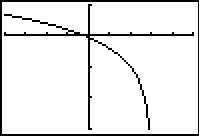
\includegraphics[width=2in]{./ExpLogsGraphics/Intro01.jpg} &

\hspace{1in} 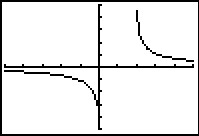
\includegraphics[width=2in]{./ExpLogsGraphics/Intro02.jpg} \\

$y = f(x) = 2\log(3-x)-1$ & 

\hspace{1in} $y = g(x) = \ln \left(\dfrac{x}{x-1}\right)$ \\

\end{tabular}

\end{center}

\vspace{-0.25in} \qed

\end{ex}

While logarithms have some interesting applications of their own which you'll explore in the exercises, their primary use to us will be to undo exponential functions. (This is, after all, how they were defined.)  Our last example solidifies this and reviews all of the material in the section.

\begin{ex}  Let $f(x) = 2^{x-1} - 3$. \label{proceduralinverse}

\begin{enumerate}

\item  Graph $f$ using transformations and state the domain and range of $f$.

\item  Explain why $f$ is invertible and find a formula for $f^{-1}(x)$.

\item  Graph $f^{-1}$ using transformations and state the domain and range of $f^{-1}$.

\item  Verify $\left(f^{-1} \circ f\right)(x) = x$ for all $x$ in the domain of $f$ and  $\left(f \circ f^{-1} \right)(x) = x$ for all $x$ in the domain of $f^{-1}$.

\item  Graph $f$ and $f^{-1}$ on the same set of axes and check the symmetry about the line $y = x$.

\end{enumerate}

{\bf Solution.}  

\begin{enumerate}

\item  If we identify $g(x) = 2^{x}$, we see $f(x) = g(x-1)-3$.  We pick the points $\left(-1, \frac{1}{2}\right)$, $(0,1)$ and $(1, 2)$ on the graph of $g$ along with the horizontal asymptote $y=0$ to track through the transformations. By Theorem \ref{transformationsthm} we first add $1$ to the $x$-coordinates of the points on the graph of $g$ (shifting $g$ to the right $1$ unit) to get $\left(0, \frac{1}{2}\right)$, $(1,1)$ and $(2, 2)$.  The horizontal asymptote remains $y=0$.  Next, we subtract $3$ from the $y$-coordinates, shifting the graph down $3$ units.  We get the points $\left(0, -\frac{5}{2}\right)$, $(1,-2)$ and $(2, -1)$ with the horizontal asymptote now at $y=-3$.  Connecting the dots in the order and manner as they were on the graph of $g$, we get the graph below.  We see that the domain of $f$ is the same as $g$, namely $(-\infty, \infty)$, but that the range of $f$ is $(-3, \infty)$.


\[\begin{array}{ccc}

\begin{mfpic}[10][8]{-4}{5}{-3.25}{8.25}
\point[2pt]{(-1,0.5), (0,1), (1,2)}
\axes
\tlabel[cc](5,-0.5){\scriptsize $x$}
\tlabel[cc](0.5,8.25){\scriptsize $y$}
\tcaption{\scriptsize $y = h(x) = 2^{x}$}
\xmarks{-3,-2,-1,1,2,3,4}
\ymarks{-3,-2,-1,1,2,3,4,5,6,7}
\tlpointsep{4pt}
\axislabels {x}{{\tiny $-3 \hspace{7pt}$} -3, {\tiny $-2 \hspace{7pt}$} -2, {\tiny $-1 \hspace{7pt}$} -1, {\tiny $1$} 1, {\tiny $2$} 2, {\tiny $3$} 3, {\tiny $4$} 4}
\axislabels {y}{{\tiny $-3$} -3, {\tiny $-2$} -2, {\tiny $-1$} -1,{\tiny $1$} 1, {\tiny $2$} 2, {\tiny $3$} 3, {\tiny $4$} 4, {\tiny $5$} 5, {\tiny $6$} 6, {\tiny $7$} 7}
\arrow \reverse \arrow \function{-3.5, 3, 0.1}{2**x}
\end{mfpic}

&

\xrightarrow{\hspace{1in}}

&

\begin{mfpic}[10][8]{-4}{5}{-3.25}{8.25}
\point[2pt]{(0,-2.5), (1,-2), (2,-1)}
\axes
\tlabel[cc](5,-0.5){\scriptsize $x$}
\tlabel[cc](0.5,8.25){\scriptsize $y$}
\tcaption{\scriptsize $y = f(x) = 2^{x-1}-3$}
\xmarks{-3,-2,-1,1,2,3,4}
\ymarks{-3,-2,-1,1,2,3,4,5,6,7}
\tlpointsep{4pt}
\axislabels {x}{{\tiny $-3 \hspace{7pt}$} -3, {\tiny $-2 \hspace{7pt}$} -2, {\tiny $-1 \hspace{7pt}$} -1, {\tiny $1$} 1, {\tiny $2$} 2, {\tiny $3$} 3, {\tiny $4$} 4}
\axislabels {y}{{\tiny $-2$} -2, {\tiny $-1$} -1,{\tiny $1$} 1, {\tiny $2$} 2, {\tiny $3$} 3, {\tiny $4$} 4, {\tiny $5$} 5, {\tiny $6$} 6, {\tiny $7$} 7}
\arrow \reverse \arrow \function{-2.5, 4, 0.1}{(2**(x-1))-3}
\dashed \polyline{(-4,-3),(5,-3)}
\end{mfpic} \\

\end{array}\]

\item  The graph of $f$ passes the Horizontal Line Test so $f$ is one-to-one, hence invertible.  To find a formula for $f^{-1}(x)$, we normally set $y=f(x)$, interchange the $x$ and $y$, then proceed to solve for $y$.  Doing so in this situation leads us to the equation $x = 2^{y-1}-3$.  We have yet to discuss how to solve this kind of equation, so we will attempt to find the formula for $f^{-1}$ from a procedural perspective.  If we break $f(x) = 2^{x-1}-3$ into a series of steps, we find $f$ takes an input $x$ and applies the steps

\begin{enumerate}

\item subtract $1$

\item put as an exponent on $2$

\item subtract $3$

\end{enumerate}

Clearly, to undo subtracting $1$, we will add $1$, and similarly we undo subtracting $3$ by adding $3$.  How do we undo the second step?  The answer is we use the logarithm.  By definition, $\log_{2}(x)$ undoes exponentiation by $2$.  Hence, $f^{-1}$ should

\begin{enumerate}

\item add $3$

\item take the logarithm base $2$

\item add $1$

\end{enumerate}

In symbols, $f^{-1}(x) = \log_{2}(x+3)+1$.  


\item  To graph $f^{-1}(x) = \log_{2}(x+3)+1$ using transformations, we start with $j(x) = \log_{2}(x)$.  We track the points $\left(\frac{1}{2},-1\right)$, $(1,0)$ and $(2, 1)$ on the graph of $j$ along with the vertical asymptote $x=0$ through the transformations using Theorem \ref{transformationsthm}.  Since $f^{-1}(x) = j(x+3)+1$, we first subtract $3$ from each of the $x$ values (including the vertical asymptote) to obtain  $\left(-\frac{5}{2},-1\right)$, $(-2,0)$ and $(-1, 1)$ with a vertical asymptote $x = -3$.  Next, we add $1$ to the $y$ values on the graph and get $\left(-\frac{5}{2},0\right)$, $(-2,1)$ and $(-1, 2)$.  If you are experiencing \textit{d\'{e}j\`{a} vu}, there is a good reason for it but we leave it to the reader to determine the source of this uncanny familiarity.  We obtain the graph below.  The domain of $f^{-1}$ is $(-3, \infty)$, which matches the range of $f$, and the range of $f^{-1}$ is $(-\infty, \infty)$, which matches the domain of $f$.

\[\begin{array}{ccc}

\begin{mfpic}[10]{-4}{9}{-4}{5}
\point[2pt]{(0.5,-1), (1,0), (2,1)}
\axes
\tlabel[cc](9,-0.5){\scriptsize $x$}
\tlabel[cc](0.5,5){\scriptsize $y$}
\tcaption{\scriptsize $y = j(x) = \log_{2}(x)$}
\ymarks{-3,-2,-1,1,2,3,4}
\xmarks{-3,-2,-1,1,2,3,4,5,6,7,8}
\tlpointsep{4pt}
\axislabels {y}{{\tiny $-3$} -3,{\tiny $-2$} -2, {\tiny $-1$} -1, {\tiny $1$} 1, {\tiny $2$} 2, {\tiny $3$} 3, {\tiny $4$} 4}
\axislabels {x}{{\tiny $-3 \hspace{7pt}$} -3, {\tiny $-2 \hspace{7pt}$} -2, {\tiny $-1 \hspace{7pt}$} -1,{\tiny $1$} 1, {\tiny $2$} 2, {\tiny $3$} 3, {\tiny $4$} 4, {\tiny $5$} 5, {\tiny $6$} 6, {\tiny $7$} 7, {\tiny $8$} 8}
\arrow \reverse \arrow \parafcn{-3.5, 3.1, 0.1}{(2**t,t)}
\end{mfpic}

&

\xrightarrow{\hspace{1in}}

&

\begin{mfpic}[10]{-4}{9}{-4}{5}
\point[2pt]{(-2.5,0), (-2,1), (-1,2)}
\axes
\tlabel[cc](9,-0.5){\scriptsize $x$}
\tlabel[cc](0.5,5){\scriptsize $y$}
\tcaption{\scriptsize $y = f^{-1}(x) = \log_{2}(x+3)+1$}
\ymarks{-3,-2,-1,1,2,3,4}
\xmarks{-3,-2,-1,1,2,3,4,5,6,7,8}
\tlpointsep{4pt}
\axislabels {y}{{\tiny $-3$} -3,{\tiny $-2$} -2, {\tiny $-1$} -1, {\tiny $1$} 1, {\tiny $2$} 2, {\tiny $3$} 3, {\tiny $4$} 4}
\axislabels {x}{{\tiny $-2 \hspace{7pt}$} -2, {\tiny $-1 \hspace{7pt}$} -1,{\tiny $1$} 1, {\tiny $2$} 2, {\tiny $3$} 3, {\tiny $4$} 4, {\tiny $5$} 5, {\tiny $6$} 6, {\tiny $7$} 7, {\tiny $8$} 8}
\arrow \reverse \arrow \parafcn{-2.5, 4.1, 0.1}{((2**(t-1))-3,t)}
\dashed \polyline{(-3,-4),(-3,5)}
\end{mfpic} \\

\end{array}\]

\item  We now verify that $f(x) = 2^{x-1}-3$ and $f^{-1}(x) = \log_{2}(x+3)+1$ satisfy the composition requirement for inverses.  For all real numbers $x$, 

\setlength{\extrarowheight}{4pt}

\[ \begin{array}{rclr}

\left(f^{-1}\circ f\right)(x) & = & f^{-1}(f(x)) & \\

& = & f^{-1}\left(2^{x-1}-3 \right) & \\

& = & \log_{2}\left( \left[2^{x-1}-3\right]+3 \right)+1 & \\

& = & \log_{2}\left( 2^{x-1} \right)+1 & \\

& = & (x-1) +1 & \mbox{ Since $\log_{2}\left(2^{u}\right) = u$ for all real numbers $u$} \\

& = & x \, \, \checkmark \\

\end{array} \]

\setlength{\extrarowheight}{2pt}

For all real numbers $x > -3$, we have\footnote{Pay attention - can you spot in which step below we need $x > -3$?} 

\setlength{\extrarowheight}{4pt}

\[ \begin{array}{rclr}

\left(f\circ f^{-1}\right)(x) & = & f\left(f^{-1}(x)\right) & \\

& = & f\left( \log_{2}(x+3)+1 \right) & \\

& = & 2^{\left( \log_{2}(x+3)+1 \right)-1} - 3 & \\

& = & 2^{\log_{2}(x+3)} - 3 & \\

& = & (x+3) -3 & \mbox{ Since $2^{\log_{2}(u)} = u$ for all real numbers $u > 0$} \\

& = & x \, \, \checkmark \\

\end{array} \]

\setlength{\extrarowheight}{2pt}

\item  Last, but certainly not least, we graph $y=f(x)$ and $y=f^{-1}(x)$ on the same set of axes and see the symmetry about the line $y=x$.

\begin{center}
\begin{mfpic}[12]{-4}{9}{-4}{9}
\axes
\tlabel[cc](9,-0.5){\scriptsize $x$}
\tlabel[cc](0.5,9){\scriptsize $y$}
\tlabel(-4,-5){$y = f(x) = 2^{x-1}-3$}
\tlabel(-4,-6){\mbox{\boldmath $y = f^{-1}(x) = \log_{2}(x+3)+1$}}
\xmarks{-3,-2,-1,1,2,3,4,5,6,7,8}
\ymarks{-3,-2,-1,1,2,3,4,5,6,7,8}
\tlpointsep{4pt}
\axislabels {x}{{\tiny $-3 \hspace{7pt}$} -3, {\tiny $-2 \hspace{7pt}$} -2, {\tiny $-1 \hspace{7pt}$} -1, {\tiny $1$} 1, {\tiny $2$} 2, {\tiny $3$} 3, {\tiny $4$} 4, {\tiny $5$} 5, {\tiny $6$} 6, {\tiny $7$} 7, {\tiny $8$} 8}
\axislabels {y}{{\tiny $-2$} -2, {\tiny $-1$} -1,{\tiny $1$} 1, {\tiny $2$} 2, {\tiny $3$} 3, {\tiny $4$} 4, {\tiny $5$} 5, {\tiny $6$} 6, {\tiny $7$} 7, {\tiny $8$} 8}
\arrow \reverse \arrow \function{-4.1, 4.1, 0.1}{(2**(x-1))-3}
\dashed \polyline{(-4,-3),(5,-3)}
\dashed \polyline{(-4,-4),(9,9)}
\dashed \polyline{(-3,-4),(-3,5)}
\penwd{1.5pt}
\arrow \reverse \arrow \parafcn{-4.1, 4.1, 0.1}{((2**(t-1))-3,t)}
\end{mfpic}

\end{center}
\end{enumerate}

\qed

\end{ex}

\newpage

\subsection{Exercises}

In Exercises \ref{rewritefirstex} - \ref{rewritelastex}, use the property: $b^{a} = c$ if and only if $\log_{b}(c) = a$ from Theorem \ref{logfcnprops} to rewrite the given equation in the other form.  That is, rewrite the exponential equations as logarithmic equations and rewrite the logarithmic equations as exponential equations.

\begin{multicols}{3}
\begin{enumerate}

\item  $2^{3} = 8$ \label{rewritefirstex}

\item  $5^{-3} = \frac{1}{125}$  

\item  $4^{5/2} = 32$  

\setcounter{HW}{\value{enumi}}
\end{enumerate}
\end{multicols}

\begin{multicols}{3}
\begin{enumerate}
\setcounter{enumi}{\value{HW}}

\item  $\left(\frac{1}{3}\right)^{-2} = 9$  

\item  $\left(\frac{4}{25}\right)^{-1/2} = \frac{5}{2}$  

\item  $10^{-3} = 0.001$ 

\setcounter{HW}{\value{enumi}}
\end{enumerate}
\end{multicols}

\begin{multicols}{3}
\begin{enumerate}
\setcounter{enumi}{\value{HW}}

\item  $e^{0}  = 1$  

\item  $\log_{5}(25) = 2$  

\item  $\log_{25} (5) = \frac{1}{2}$  

\setcounter{HW}{\value{enumi}}
\end{enumerate}
\end{multicols}

\begin{multicols}{3}
\begin{enumerate}
\setcounter{enumi}{\value{HW}}

\item  $\log_{3} \left(\frac{1}{81} \right) = -4$  

\item  $\log_{\frac{4}{3}} \left(\frac{3}{4} \right) = -1$  

\item  $\log(100) = 2$  

\setcounter{HW}{\value{enumi}}
\end{enumerate}
\end{multicols}

\begin{multicols}{3}
\begin{enumerate}
\setcounter{enumi}{\value{HW}}

\item  $\log (0.1) = -1$  

\item  $\ln(e) = 1$ 

\item  $\ln\left(\frac{1}{\sqrt{e}}\right) = -\frac{1}{2}$  \label{rewritelastex}

\setcounter{HW}{\value{enumi}}
\end{enumerate}
\end{multicols}

In Exercises \ref{simplifylogfirst} - \ref{simplifyloglast}, evaluate the expression.

\begin{multicols}{3}
\begin{enumerate}
\setcounter{enumi}{\value{HW}}

\item $\log_{3} (27)$  \label{simplifylogfirst}
\item $\log_{6} (216)$
\item $\log_{2} (32)$

\setcounter{HW}{\value{enumi}}
\end{enumerate}
\end{multicols}


\begin{multicols}{3}
\begin{enumerate}
\setcounter{enumi}{\value{HW}}

\item  $\log_{6} \left( \frac{1}{36} \right)$
\item $\log_{8} (4)$
\item $\log_{36} (216)$

\setcounter{HW}{\value{enumi}}
\end{enumerate}
\end{multicols}


\begin{multicols}{3}
\begin{enumerate}
\setcounter{enumi}{\value{HW}}

\item $\log_{\frac{1}{5}} (625)$
\item  $\log_{\frac{1}{6}} (216)$
\item $\log_{36} (36)$ 

\setcounter{HW}{\value{enumi}}
\end{enumerate}
\end{multicols}


\begin{multicols}{3}
\begin{enumerate}
\setcounter{enumi}{\value{HW}}

\item $\log \left(\frac{1}{1000000}\right)$
\item $\log(0.01)$
\item $\ln\left(e^3\right)$

\setcounter{HW}{\value{enumi}}
\end{enumerate}
\end{multicols}


\begin{multicols}{3}
\begin{enumerate}
\setcounter{enumi}{\value{HW}}

\item $\log_{4} (8)$
\item $\log_{6} (1)$
\item $\log_{13} \left(\sqrt{13}\right)$

\setcounter{HW}{\value{enumi}}
\end{enumerate}
\end{multicols}


\begin{multicols}{3}
\begin{enumerate}
\setcounter{enumi}{\value{HW}}

\item $\log_{36} \left(\sqrt[4]{36}\right)$
\item $7^{\log_{7} (3)}$
\item  $36^{\log_{36}(216)}$

\setcounter{HW}{\value{enumi}}
\end{enumerate}
\end{multicols}


\begin{multicols}{3}
\begin{enumerate}
\setcounter{enumi}{\value{HW}}

\item  $\log_{36} \left(36^{216}\right)$
\item $\ln \left(e^{5} \right)$
\item $\log \left(\sqrt[9]{10^{11}}\right)$

\setcounter{HW}{\value{enumi}}
\end{enumerate}
\end{multicols}


\begin{multicols}{3}
\begin{enumerate}
\setcounter{enumi}{\value{HW}}

\item  $\log\left( \sqrt[3]{10^5} \right)$
\item  $\ln \left( \frac{1}{\sqrt{e}}\right)$
\item $\log_{5} \left(3^{\log_{3} (5)}\right)$

\setcounter{HW}{\value{enumi}}
\end{enumerate}
\end{multicols}


\begin{multicols}{3}
\begin{enumerate}
\setcounter{enumi}{\value{HW}}

\item $\log\left(e^{\ln(100)}\right)$ 
\item $\log_{2}\left(3^{-\log_{3}(2)}\right)$
\item $\ln\left(42^{6\log(1)}\right)$ \label{simplifyloglast}

\setcounter{HW}{\value{enumi}}
\end{enumerate}
\end{multicols}

In Exercises \ref{domainlogfirst} - \ref{domainloglast}, find the domain of the function.

\begin{multicols}{2}
\begin{enumerate}
\setcounter{enumi}{\value{HW}}


\item $f(x) = \ln(x^{2} + 1)$ \label{domainlogfirst}
\item $f(x) = \log_{7}(4x + 8)$

\setcounter{HW}{\value{enumi}}
\end{enumerate}
\end{multicols}

\begin{multicols}{2}
\begin{enumerate}
\setcounter{enumi}{\value{HW}}


\item $f(x) = \ln(4x-20)$
\item $f(x) = \log \left(x^2+9x+18\right)$

\setcounter{HW}{\value{enumi}}
\end{enumerate}
\end{multicols}

\begin{multicols}{2}
\begin{enumerate}
\setcounter{enumi}{\value{HW}}

\item $f(x) = \log \left(\dfrac{x + 2}{x^{2} - 1}\right)$
\item $f(x) = \log\left(\dfrac{x^2+9x+18}{4x-20}\right)$

\setcounter{HW}{\value{enumi}}
\end{enumerate}
\end{multicols}

\begin{multicols}{2}
\begin{enumerate}
\setcounter{enumi}{\value{HW}}

\item $f(x) = \ln(7 - x) + \ln(x - 4)$
\item $f(x) = \ln(4x-20) + \ln\left(x^2+9x+18\right)$

\setcounter{HW}{\value{enumi}}
\end{enumerate}
\end{multicols}

\begin{multicols}{2}
\begin{enumerate}
\setcounter{enumi}{\value{HW}}

\item $f(x) = \log\left(x^2+x+1\right)$
\item $f(x) = \sqrt[4]{\log_{4} (x)}$

\setcounter{HW}{\value{enumi}}
\end{enumerate}
\end{multicols}

\begin{multicols}{2}
\begin{enumerate}
\setcounter{enumi}{\value{HW}}

\item $f(x) = \log_{9}(|x + 3| - 4)$
\item $f(x) = \ln(\sqrt{x - 4} - 3)$

\setcounter{HW}{\value{enumi}}
\end{enumerate}
\end{multicols}

\begin{multicols}{2}
\begin{enumerate}
\setcounter{enumi}{\value{HW}}

\item $f(x) = \dfrac{1}{3 - \log_{5} (x)}$
\item $f(x) = \dfrac{\sqrt{-1 - x}}{\log_{\frac{1}{2}} (x)}$

\setcounter{HW}{\value{enumi}}
\end{enumerate}
\end{multicols}

\begin{multicols}{2}
\begin{enumerate}
\setcounter{enumi}{\value{HW}}

\item $f(x) = \ln(-2x^{3} - x^{2} + 13x - 6)$  \label{domainloglast}

\setcounter{HW}{\value{enumi}}
\end{enumerate}
\end{multicols}

In Exercises \ref{graphexpfirst} - \ref{graphexplast}, sketch the graph of $y=g(x)$ by starting with the graph of $y = f(x)$ and using transformations.  Track at least three points of your choice and the horizontal asymptote through the transformations. State the domain and range of $g$.

\begin{multicols}{2}
\begin{enumerate}
\setcounter{enumi}{\value{HW}}


\item  $f(x) = 2^{x}$, $g(x) = 2^{x} - 1$ \label{graphexpfirst}

\item  $f(x) = \left(\frac{1}{3}\right)^{x}$, $g(x) = \left(\frac{1}{3}\right)^{x-1}$

\setcounter{HW}{\value{enumi}}
\end{enumerate}
\end{multicols}

\begin{multicols}{2}
\begin{enumerate}
\setcounter{enumi}{\value{HW}}

\item  $f(x) = 3^{x}$, $g(x) = 3^{-x}+2$

\item  $f(x) = 10^{x}$, $g(x) = 10^{\frac{x+1}{2}} - 20$  

\setcounter{HW}{\value{enumi}}
\end{enumerate}
\end{multicols}

\begin{multicols}{2}
\begin{enumerate}
\setcounter{enumi}{\value{HW}}

\item  $f(x) = e^{x}$, $g(x) = 8 - e^{-x}$

\item  $f(x) = e^{x}$, $g(x) = 10e^{-0.1x}$ \label{graphexplast}

\setcounter{HW}{\value{enumi}}
\end{enumerate}
\end{multicols}


In Exercises \ref{graphlogfirst} - \ref{graphloglast}, sketch the graph of $y=g(x)$ by starting with the graph of $y = f(x)$ and using transformations.  Track at least three points of your choice and the vertical asymptote through the transformations. State the domain and range of $g$.


\begin{multicols}{2}
\begin{enumerate}
\setcounter{enumi}{\value{HW}}

\item  $f(x) = \log_{2}(x)$, $g(x) = \log_{2}(x+1)$ \label{graphlogfirst}

\item  $f(x) = \log_{\frac{1}{3}}(x)$, $g(x) = \log_{\frac{1}{3}}(x)+1$

\setcounter{HW}{\value{enumi}}
\end{enumerate}
\end{multicols}

\begin{multicols}{2}
\begin{enumerate}
\setcounter{enumi}{\value{HW}}


\item  $f(x) = \log_{3}(x)$, $g(x) = -\log_{3}(x-2)$

\item  $f(x) = \log(x)$, $g(x) = 2\log(x+20) -1$  

\setcounter{HW}{\value{enumi}}
\end{enumerate}
\end{multicols}

\begin{multicols}{2}
\begin{enumerate}
\setcounter{enumi}{\value{HW}}


\item  $f(x) = \ln(x)$, $g(x) = -\ln(8-x)$

\item  $f(x) = \ln(x)$, $g(x) = -10\ln\left(\frac{x}{10}\right)$ \label{graphloglast}

\setcounter{HW}{\value{enumi}}
\end{enumerate}
\end{multicols}

\begin{enumerate}
\setcounter{enumi}{\value{HW}}

\smallskip

\item  Verify that each function in Exercises \ref{graphlogfirst} - \ref{graphloglast} is the inverse of the corresponding function in Exercises \ref{graphexpfirst} - \ref{graphexplast}.  (Match up \#\ref{graphexpfirst} and \#\ref{graphlogfirst}, and so on.)

\setcounter{HW}{\value{enumi}}
\end{enumerate}

In Exercises \ref{inverselogexpfirst} - \ref{inverselogexplast},  find the inverse of the function from the `procedural perspective' discussed in Example \ref{proceduralinverse} and graph the function and its inverse on the same set of axes.

\begin{multicols}{2}
\begin{enumerate}
\setcounter{enumi}{\value{HW}}

\item $f(x) = 3^{x + 2} - 4$  \label{inverselogexpfirst} 
\item $f(x) = \log_{4}(x - 1)$

\setcounter{HW}{\value{enumi}}
\end{enumerate}
\end{multicols}

\enlargethispage{.5in}
\vspace{-.2in}

\begin{multicols}{2}
\begin{enumerate}
\setcounter{enumi}{\value{HW}}

\item $f(x) = -2^{-x} + 1$
\item $f(x) = 5\log(x) - 2$ \label{inverselogexplast}

\setcounter{HW}{\value{enumi}}
\end{enumerate}
\end{multicols}
\vspace{-.2in}

\pagebreak

\phantomsection
\label{logarithmicscales}

(Logarithmic Scales) In Exercises \ref{Richterexercise} - \ref{pHexercise}, we introduce three widely used measurement scales which involve common logarithms: the Richter scale, the decibel scale and the pH scale.  The computations involved in all three scales are nearly identical so pay attention to the subtle differences. \index{logarithmic scales}

\begin{enumerate}
\setcounter{enumi}{\value{HW}}

\item \label{Richterexercise} \index{Richter Scale} \index{earthquake ! Richter Scale} Earthquakes are complicated events and it is not our intent to provide a complete discussion of the science involved in them.  Instead, we refer the interested reader to a solid course in Geology\footnote{Rock-solid, perhaps?} or the U.S. Geological Survey's Earthquake Hazards Program found \href{http://earthquake.usgs.gov/}{\underline{here}} and present only a simplified version of the \href{http://en.wikipedia.org/wiki/Richter_scale}{\underline{Richter scale}}.  The Richter scale measures the magnitude of an earthquake by comparing the amplitude of the seismic waves of the given earthquake to those of a ``magnitude 0 event'', which was chosen to be a seismograph reading of $0.001$ millimeters recorded on a seismometer 100 kilometers from the earthquake's epicenter.  Specifically, the magnitude of an earthquake is given by \[M(x) = \log \left(\dfrac{x}{0.001}\right)\] where $x$ is the seismograph reading in millimeters of the earthquake recorded 100 kilometers from the epicenter.  

\begin{enumerate}

\item Show that $M(0.001) = 0$.
\item Compute $M(80,000)$.
\item Show that an earthquake which registered 6.7 on the Richter scale had a seismograph reading ten times larger than one which measured 5.7.
\item Find two news stories about recent earthquakes which give their magnitudes on the Richter scale.  How many times larger was the seismograph reading of the earthquake with larger magnitude?

\end{enumerate}

\item \label{decibelexercise} \index{decibel} \index{sound intensity level ! decibel} While the decibel scale can be used in many disciplines,\footnote{See this  \href{http://en.wikipedia.org/wiki/Decibel}{\underline{webpage}} for more information.} we shall restrict our attention to its use in acoustics, specifically its use in measuring the intensity level of sound.\footnote{As of the writing of this exercise, the Wikipedia page given \href{http://en.wikipedia.org/wiki/Sound_intensity_level}{\underline{here}} states that it may not meet the ``general notability guideline'' nor does it cite any references or sources.  I find this odd because it is this very usage of the decibel scale which shows up in every College Algebra book I have read.  Perhaps those other books have been wrong all along and we're just blindly following tradition.}  The Sound Intensity Level $L$ (measured in decibels) of a sound intensity $I$ (measured in watts per square meter) is given by \[L(I) = 10\log\left( \dfrac{I}{10^{-12}} \right).\] Like the Richter scale, this scale compares $I$ to baseline: $10^{-12} \frac{W}{m^{2}}$ is the threshold of human hearing. 

\begin{enumerate}

\item Compute $L(10^{-6})$.
\item Damage to your hearing can start with short term exposure to sound levels around 115 decibels.  What intensity $I$ is needed to produce this level? 
\item Compute $L(1)$.  How does this compare with the threshold of pain which is around 140 decibels?

\end{enumerate}

\item \label{pHexercise} \index{pH} \index{acidity of a solution ! pH} \index{alkalinity of a solution ! pH} The pH of a solution is a measure of its acidity or alkalinity.  Specifically, $\mbox{pH} = -\log[\mbox{H}^{+}]$ where $[\mbox{H}^{+}]$ is the hydrogen ion concentration in moles per liter.  A solution with a pH less than 7 is an acid, one with a pH greater than 7 is a base (alkaline) and a pH of 7 is regarded as neutral.

\begin{enumerate}

\item The hydrogen ion concentration of pure water is $[\mbox{H}^{+}] = 10^{-7}$.  Find its pH.
\item Find the pH of a solution with $[\mbox{H}^{+}] = 6.3 \times 10^{-13}$.
\item The pH of gastric acid (the acid in your stomach) is about $0.7$.  What is the corresponding hydrogen ion concentration?

\end{enumerate}

\setcounter{HW}{\value{enumi}}
\end{enumerate}

\begin{enumerate}
\setcounter{enumi}{\value{HW}}

\item Show that $\log_{b} 1 = 0$ and $\log_{b} b = 1$ for every $b > 0, \; b \neq 1$.

\item (Crazy bonus question) Without using your calculator, determine which is larger: $e^{\pi}$ or $\pi^{e}$.

\setcounter{HW}{\value{enumi}}
\end{enumerate}


\newpage

\subsection{Answers}

\begin{multicols}{3}
\begin{enumerate}

\item $\log_{2}(8) = 3$

\item  $\log_{5}\left(\frac{1}{125}\right) = -3$

\item  $\log_{4}(32) = \frac{5}{2}$

\setcounter{HW}{\value{enumi}}
\end{enumerate}
\end{multicols}

\begin{multicols}{3}
\begin{enumerate}
\setcounter{enumi}{\value{HW}}


\item  $\log_{\frac{1}{3}}(9) = -2$

\item  $\log_{\frac{4}{25}}\left(\frac{5}{2}\right) = -\frac{1}{2}$

\item  $\log(0.001) = -3$

\setcounter{HW}{\value{enumi}}
\end{enumerate}
\end{multicols}

\begin{multicols}{3}
\begin{enumerate}
\setcounter{enumi}{\value{HW}}


\item  $\ln(1) = 0$

\item  $5^{2} = 25$

\item  $(25)^{\frac{1}{2}} = 5$

\setcounter{HW}{\value{enumi}}
\end{enumerate}
\end{multicols}

\begin{multicols}{3}
\begin{enumerate}
\setcounter{enumi}{\value{HW}}


\item  $3^{-4} = \frac{1}{81}$

\item  $\left(\frac{4}{3} \right)^{-1} = \frac{3}{4}$

\item  $10^{2} = 100$

\setcounter{HW}{\value{enumi}}
\end{enumerate}
\end{multicols}

\begin{multicols}{3}
\begin{enumerate}
\setcounter{enumi}{\value{HW}}


\item  $10^{-1} = 0.1$

\item  $e^{1} = e$

\item  $e^{-\frac{1}{2}} = \frac{1}{\sqrt{e}}$

\setcounter{HW}{\value{enumi}}
\end{enumerate}
\end{multicols}

\begin{multicols}{3}
\begin{enumerate}
\setcounter{enumi}{\value{HW}}

\item $\log_{3} (27) = 3$
\item $\log_{6} (216) = 3$
\item $\log_{2} (32) = 5$

\setcounter{HW}{\value{enumi}}
\end{enumerate}
\end{multicols}

\begin{multicols}{3}
\begin{enumerate}
\setcounter{enumi}{\value{HW}}


\item  $\log_{6} \left( \frac{1}{36} \right) = -2$
\item $\log_{8} (4) = \frac{2}{3}$
\item $\log_{36} (216) = \frac{3}{2}$

\setcounter{HW}{\value{enumi}}
\end{enumerate}
\end{multicols}

\begin{multicols}{3}
\begin{enumerate}
\setcounter{enumi}{\value{HW}}


\item $\log_{\frac{1}{5}} (625) = -4$
\item  $\log_{\frac{1}{6}} (216) = -3$
\item $\log_{36} (36)=1$ 

\setcounter{HW}{\value{enumi}}
\end{enumerate}
\end{multicols}

\begin{multicols}{3}
\begin{enumerate}
\setcounter{enumi}{\value{HW}}


\item $\log \frac{1}{1000000} = -6$
\item $\log(0.01) = -2$
\item $\ln\left(e^3\right) = 3$

\setcounter{HW}{\value{enumi}}
\end{enumerate}
\end{multicols}

\begin{multicols}{3}
\begin{enumerate}
\setcounter{enumi}{\value{HW}}


\item $\log_{4} (8) = \frac{3}{2}$
\item $\log_{6} (1) = 0$
\item $\log_{13} \left(\sqrt{13}\right) = \frac{1}{2}$

\setcounter{HW}{\value{enumi}}
\end{enumerate}
\end{multicols}

\begin{multicols}{3}
\begin{enumerate}
\setcounter{enumi}{\value{HW}}


\item $\log_{36} \left(\sqrt[4]{36}\right) = \frac{1}{4}$
\item $7^{\log_{7} (3)} = 3$
\item  $36^{\log_{36}(216)} = 216$

\setcounter{HW}{\value{enumi}}
\end{enumerate}
\end{multicols}

\begin{multicols}{3}
\begin{enumerate}
\setcounter{enumi}{\value{HW}}


\item  $\log_{36} \left(36^{216}\right) = 216$
\item $\ln(e^{5}) = 5$
\item $\log \left(\sqrt[9]{10^{11}}\right) = \frac{11}{9}$

\setcounter{HW}{\value{enumi}}
\end{enumerate}
\end{multicols}

\begin{multicols}{3}
\begin{enumerate}
\setcounter{enumi}{\value{HW}}


\item  $\log\left( \sqrt[3]{10^5} \right) = \frac{5}{3}$
\item  $\ln \left( \frac{1}{\sqrt{e}}\right) = -\frac{1}{2} $
\item $\log_{5} \left(3^{\log_{3} 5}\right) = 1$

\setcounter{HW}{\value{enumi}}
\end{enumerate}
\end{multicols}

\begin{multicols}{3}
\begin{enumerate}
\setcounter{enumi}{\value{HW}}


\item $\log\left(e^{\ln(100)}\right) = 2$
\item $\log_{2}\left(3^{-\log_{3}(2)}\right) = -1$
\item $\ln\left(42^{6\log(1)}\right) = 0$

\setcounter{HW}{\value{enumi}}
\end{enumerate}
\end{multicols}


\begin{multicols}{3}
\begin{enumerate}
\setcounter{enumi}{\value{HW}}


\item $(-\infty, \infty)$
\item $(-2, \infty)$
\item $(5, \infty)$

\setcounter{HW}{\value{enumi}}
\end{enumerate}
\end{multicols}


\begin{multicols}{3}
\begin{enumerate}
\setcounter{enumi}{\value{HW}}


\item $(-\infty, -6) \cup (-3, \infty)$
\item $(-2, -1) \cup (1, \infty)$
\item $(-6,-3) \cup (5, \infty)$

\setcounter{HW}{\value{enumi}}
\end{enumerate}
\end{multicols}


\begin{multicols}{3}
\begin{enumerate}
\setcounter{enumi}{\value{HW}}


\item $(4, 7)$
\item $(5, \infty)$
\item $(-\infty, \infty)$

\setcounter{HW}{\value{enumi}}
\end{enumerate}
\end{multicols}


\begin{multicols}{3}
\begin{enumerate}
\setcounter{enumi}{\value{HW}}


\item $[1, \infty)$
\item $(-\infty, -7) \cup (1, \infty)$
\item $(13, \infty)$

\setcounter{HW}{\value{enumi}}
\end{enumerate}
\end{multicols}


\begin{multicols}{3}
\begin{enumerate}
\setcounter{enumi}{\value{HW}}


\item $(0, 125) \cup (125, \infty)$
\item No domain
\item $(-\infty, -3) \cup \left(\frac{1}{2}, 2\right)$

\setcounter{HW}{\value{enumi}}
\end{enumerate}
\end{multicols}

\pagebreak

\begin{multicols}{2}
\begin{enumerate}
\setcounter{enumi}{\value{HW}}

\item  Domain of $g$:  $(-\infty, \infty)$\\
 Range of $g$:  $(-1, \infty)$\\
 
\begin{mfpic}[10]{-4}{4}{-2}{9}
\point[3pt]{(-1,-0.5), (0,0), (1,1)}
\axes
\tlabel[cc](4,-0.5){\scriptsize $x$}
\tlabel[cc](0.5,9){\scriptsize $y$}
\tcaption{\scriptsize $y = g(x) = 2^{x}-1$}
\xmarks{-3,-2,-1,1,2,3}
\ymarks{-1,1,2,3,4,5,6,7,8}
\tlabel[cc](-3,0.5){\tiny $-3 \hspace{7pt}$}
\tlabel[cc](-2,0.5){\tiny $-2 \hspace{7pt}$}
\tlabel[cc](-1,0.5){\tiny $-1 \hspace{7pt}$}
\tlabel[cc](2,-1.5){\tiny H.A. $y=-1$}
\tlpointsep{4pt}
\axislabels {x}{{\tiny $1$} 1, {\tiny $2$} 2, {\tiny $3$} 3}
\axislabels {y}{{\tiny $1$} 1, {\tiny $2$} 2, {\tiny $3$} 3, {\tiny $4$} 4, {\tiny $5$} 5, {\tiny $6$} 6, {\tiny $7$} 7, {\tiny $8$} 8}
\arrow \reverse \arrow \function{-3.5, 3.1, 0.1}{(2**(x))-1}
\dashed \polyline{(-4,-1),(4,-1)}
\end{mfpic}

\vfill

\columnbreak

\item  Domain of $g$:  $(-\infty, \infty)$ \\
 Range of $g$:  $(0, \infty)$ \\
 
\begin{mfpic}[10]{-4}{4}{-1}{10}
\point[3pt]{(0,3), (1,1), (2,0.3333)}
\axes
\tlabel[cc](4,-0.5){\scriptsize $x$}
\tlabel[cc](0.5,10){\scriptsize $y$}
\tcaption{\scriptsize $y = g(x) = \left(\frac{1}{3}\right)^{x-1}$}
\xmarks{-3,-2,-1,1,2,3}
\ymarks{1,2,3,4,5,6,7,8,9}
\tlpointsep{4pt}
\axislabels {x}{{\tiny $-3 \hspace{7pt}$} -3, {\tiny $-2 \hspace{7pt}$} -2, {\tiny $-1 \hspace{7pt}$} -1, {\tiny $1$} 1, {\tiny $2$} 2, {\tiny $3$} 3}
\axislabels {y}{{\tiny $1$} 1, {\tiny $2$} 2, {\tiny $3$} 3, {\tiny $4$} 4, {\tiny $5$} 5, {\tiny $6$} 6, {\tiny $7$} 7, {\tiny $8$} 8, {\tiny $9$} 9}
\arrow \reverse \arrow \function{-1.05, 3.5, 0.1}{3**(1-x)}
\end{mfpic} 

\setcounter{HW}{\value{enumi}}
\end{enumerate}
\end{multicols}

\begin{multicols}{2}
\begin{enumerate}
\setcounter{enumi}{\value{HW}}

\item  Domain of $g$:  $(-\infty, \infty)$\\
 Range of $g$:  $(2, \infty)$\\
 

\begin{mfpic}[10]{-4}{4}{-1}{12}
\point[3pt]{(1,2.3333), (0,3), (-1,5)}
\axes
\tlabel[cc](4,-0.5){\scriptsize $x$}
\tlabel[cc](0.5,12){\scriptsize $y$}
\tcaption{\scriptsize $y = g(x) = 3^{-x}+2$}
\xmarks{-3,-2,-1,1,2,3}
\ymarks{1,2,3,4,5,6,7,8,9,10,11}
\tlabel[cc](2,1){\tiny H.A. $y=2$}
\tlpointsep{4pt}
\axislabels {x}{{\tiny $-3 \hspace{7pt}$} -3, {\tiny $-2 \hspace{7pt}$} -2, {\tiny $-1 \hspace{7pt}$} -1, {\tiny $1$} 1, {\tiny $2$} 2, {\tiny $3$} 3}
\axislabels {y}{{\tiny $1$} 1, {\tiny $2$} 2, {\tiny $3$} 3, {\tiny $4$} 4, {\tiny $5$} 5, {\tiny $6$} 6, {\tiny $7$} 7, {\tiny $8$} 8, {\tiny $9$} 9, {\tiny $10$} 10, {\tiny $11$} 11}
\arrow \reverse \arrow \function{-2.05, 2.5, 0.1}{2+3**(0-x)}
\dashed \polyline{(-4,2),(4,2)}
\end{mfpic}

\vfill

\columnbreak

\item  Domain of $g$:  $(-\infty, \infty)$\\
 Range of $g$:  $(-20, \infty)$\\
 
\begin{mfpic}[10]{-3}{4}{-2}{9}
\point[3pt]{(-1,-1.9), (1,-1), (3,8)}
\axes
\tlabel[cc](4,-0.5){\scriptsize $x$}
\tlabel[cc](0.5,9){\scriptsize $y$}
\tcaption{\scriptsize $y = g(x) = 10^{\frac{x+1}{2}}-20$}
\xmarks{-3,-2,-1,1,2,3}
\ymarks{-2,-1,1,2,3,4,5,6,7,8}
\tlabel[cc](2,-2.5){\tiny H.A. $y=-20$}
\tlpointsep{4pt}
\axislabels {x}{{\tiny $-3 \hspace{7pt}$} -3, {\tiny $-2 \hspace{7pt}$} -2,  {\tiny $1$} 1, {\tiny $2$} 2, {\tiny $3$} 3}
\axislabels {y}{{\tiny $-10$} -1,{\tiny $10$} 1, {\tiny $20$} 2, {\tiny $30$} 3, {\tiny $40$} 4, {\tiny $50$} 5, {\tiny $60$} 6, {\tiny $70$} 7, {\tiny $80$} 8}
\arrow \reverse \arrow \function{-3, 3.06, 0.1}{((10**((x+1)/2))-20)/10}
\dashed \polyline{(-4,-2), (4,-2)}
\end{mfpic}

\setcounter{HW}{\value{enumi}}
\end{enumerate}
\end{multicols}

\begin{multicols}{2}
\begin{enumerate}
\setcounter{enumi}{\value{HW}}

\item  Domain of $g$:  $(-\infty, \infty)$\\
 Range of $g$:  $(-\infty, 8)$ \\
 
\begin{mfpic}[10]{-4}{4}{-1}{9}
\point[3pt]{(1,7.6321), (0,7), (-1,5.282)}
\axes
\tlabel[cc](4,-0.5){\scriptsize $x$}
\tlabel[cc](0.5,9){\scriptsize $y$}
\tlabel[cc](3,6){\tiny H.A. $y=8$}
\tcaption{\scriptsize $y = g(x) = 8-e^{-x}$}
\xmarks{-3,-2,-1,1,2,3}
\ymarks{1,2,3,4,5,6,7,8}
\tlpointsep{4pt}
\axislabels {x}{{\tiny $-3 \hspace{7pt}$} -3, {\tiny $-2 \hspace{7pt}$} -2, {\tiny $-1 \hspace{7pt}$} -1, {\tiny $1$} 1, {\tiny $2$} 2, {\tiny $3$} 3}
\axislabels {y}{{\tiny $1$} 1, {\tiny $2$} 2, {\tiny $3$} 3, {\tiny $4$} 4, {\tiny $5$} 5, {\tiny $6$} 6, {\tiny $7$} 7, {\tiny $8$} 8}
\arrow \reverse \arrow \function{-2.25, 2, 0.1}{8-exp(0-x)}
\dashed \polyline{(-4,8), (4,8)}
\end{mfpic}

\vfill

\columnbreak


\item  Domain of $g$:  $(-\infty, \infty)$\\
 Range of $g$:  $(0, \infty)$\\
 
\begin{mfpic}[10]{-4}{4}{-1}{9}
\point[3pt]{(1,0.3679), (0,1), (-1,2.718)}
\axes
\tlabel[cc](4,-0.5){\scriptsize $x$}
\tlabel[cc](0.5,9){\scriptsize $y$}
\tcaption{\scriptsize $y = g(x) = 10e^{-0.1x}$}
\xmarks{-3,-2,-1,1,2,3}
\ymarks{1,2,3,4,5,6,7,8}
\tlpointsep{4pt}
\axislabels {x}{{\tiny $-10 \hspace{7pt}$} -1, {\tiny $10$} 1, {\tiny $20$} 2, {\tiny $30$} 3}
\axislabels {y}{{\tiny $10$} 1, {\tiny $20$} 2, {\tiny $30$} 3, {\tiny $40$} 4, {\tiny $50$} 5, {\tiny $60$} 6, {\tiny $70$} 7, {\tiny $80$} 8}
\arrow \reverse \arrow \function{-2.15, 2, 0.1}{exp(0-x)}
\end{mfpic}

\setcounter{HW}{\value{enumi}}
\end{enumerate}
\end{multicols}

\begin{multicols}{2}
\begin{enumerate}
\setcounter{enumi}{\value{HW}}


\item  Domain of $g$: $(-1, \infty)$\\
 Range of $g$:  $(-\infty, \infty)$ \\

\begin{mfpic}[10]{-2}{9}{-4}{4}
\point[3pt]{(-0.5, -1), (0,0), (1,1)}
\axes
\tlabel[cc](0.5,4){\scriptsize $y$}
\tlabel[cc](9,-0.5){\scriptsize $x$}
\tlabel[cc](0.6, -3.1){\tiny $-3$}
\tlabel[cc](0.6, -2.1){\tiny $-2$}
\tlabel[cc](0.6, -1.1){\tiny $-1$}
\tcaption{\scriptsize $y = g(x) = \log_{2}(x+1)$}
\ymarks{-3,-2,-1,1,2,3}
\xmarks{-1,1,2,3,4,5,6,7,8}
\tlabel[cc](2,-4){\tiny V.A. $x=-1$}
\tlpointsep{4pt}
\axislabels {y}{{\tiny $1$} 1, {\tiny $2$} 2, {\tiny $3$} 3}
\axislabels {x}{{\tiny $1$} 1, {\tiny $2$} 2, {\tiny $3$} 3, {\tiny $4$} 4, {\tiny $5$} 5, {\tiny $6$} 6, {\tiny $7$} 7, {\tiny $8$} 8}
\arrow \reverse \arrow \parafcn{-3.5, 3.1, 0.1}{((2**(t))-1,t)}
\dashed \polyline{(-1,-3),(-1,4)}
\end{mfpic}

\vfill

\columnbreak

\item  Domain of $g$:  $(0, \infty)$\\
 Range of $g$:  $(-\infty, \infty)$ \\

\begin{mfpic}[10]{-1}{10}{-4}{4}
\point[3pt]{(3,0), (1,1), (0.3333,2)}
\axes
\tlabel[cc](0.5, 4){\scriptsize $y$}
\tlabel[cc](10,-0.5){\scriptsize $x$}
\tcaption{\scriptsize $y = g(x) = \log_{\frac{1}{3}}(x)+1$}
\ymarks{-3,-2,-1,1,2,3}
\xmarks{1,2,3,4,5,6,7,8,9}
\tlpointsep{4pt}
\axislabels {y}{{\tiny $-3$} -3, {\tiny $-2$} -2, {\tiny $-1$} -1, {\tiny $1$} 1, {\tiny $2$} 2, {\tiny $3$} 3}
\axislabels {x}{{\tiny $1$} 1, {\tiny $2$} 2, {\tiny $3$} 3, {\tiny $4$} 4, {\tiny $5$} 5, {\tiny $6$} 6, {\tiny $7$} 7, {\tiny $8$} 8, {\tiny $9$} 9}
\arrow \reverse \arrow \parafcn{-1.05, 3.5, 0.1}{(3**(1-t),t)}
\end{mfpic} 

\setcounter{HW}{\value{enumi}}
\end{enumerate}
\end{multicols}

\begin{multicols}{2}
\begin{enumerate}
\setcounter{enumi}{\value{HW}}


\item  Domain of $g$: $(2, \infty)$\\
 Range of $g$:  $(-\infty, \infty)$ \\
 
\begin{mfpic}[10]{-1}{12}{-4}{4}
\point[3pt]{(2.3333,1), (3,0), (5,-1)}
\axes
\tlabel[cc](0.5,4){\scriptsize $y$}
\tlabel[cc](12,-0.5){\scriptsize $x$}
\tcaption{\scriptsize $y = g(x) = -\log_{3}(x-2)$}
\ymarks{-3,-2,-1,1,2,3}
\xmarks{1,2,3,4,5,6,7,8,9,10,11}
\tlabel[cc](2,-4){\tiny V.A. $x=2$}
\tlpointsep{4pt}
\axislabels {y}{{\tiny $-3$} -3, {\tiny $-2$} -2, {\tiny $-1$} -1, {\tiny $1$} 1, {\tiny $2$} 2, {\tiny $3$} 3}
\axislabels {x}{{\tiny $1$} 1, {\tiny $2$} 2, {\tiny $3$} 3, {\tiny $4$} 4, {\tiny $5$} 5, {\tiny $6$} 6, {\tiny $7$} 7, {\tiny $8$} 8, {\tiny $9$} 9, {\tiny $10$} 10, {\tiny $11$} 11}
\arrow \reverse \arrow \parafcn{-2.05, 2.5, 0.1}{(2+3**(0-t),t)}
\dashed \polyline{(2,-3),(2,4)}
\end{mfpic} 

\vfill

\columnbreak




\item  Domain of $g$: $(-20, \infty)$\\
 Range of $g$:  $(-\infty, \infty)$\\

\begin{mfpic}[10]{-2}{11}{-3}{4}
\point[3pt]{(-1.9,-1), (-1,1), (8,3)}
\axes
\tlabel[cc](0.5,4){\scriptsize $y$}
\tlabel[cc](11,-0.5){\scriptsize $x$}
\tcaption{\scriptsize $y = g(x) = 2\log(x+20) -1$}
\ymarks{-3,-2,-1,1,2,3}
\xmarks{-2,-1,1,2,3,4,5,6,7,8,9,10}
\tlabel[cc](3,-3){\tiny V.A. $x=-20$}
\tlpointsep{4pt}
\axislabels {y}{{\tiny $-3$} -3, {\tiny $-2$} -2,  {\tiny $1$} 1, {\tiny $2$} 2, {\tiny $3$} 3}
\axislabels {x}{{\tiny $-10 \hspace{5pt}$} -1,{\tiny $10$} 1, {\tiny $20$} 2, {\tiny $30$} 3, {\tiny $40$} 4, {\tiny $50$} 5, {\tiny $60$} 6, {\tiny $70$} 7, {\tiny $80$} 8, {\tiny $90$} 9, {\tiny $100$} 10}
\arrow \reverse \arrow \parafcn{-3, 3.06, 0.1}{(((10**((t+1)/2))-20)/10,t)}
\dashed \polyline{(-2,-3), (-2,4)}
\end{mfpic}

\setcounter{HW}{\value{enumi}}
\end{enumerate}
\end{multicols}

\begin{multicols}{2}
\begin{enumerate}
\setcounter{enumi}{\value{HW}}


\item  Domain of $g$:  $(-\infty, 8)$\\
 Range of $g$:$(-\infty, \infty)$\\

\begin{mfpic}[10]{-1}{9}{-4}{4}
\point[3pt]{(7.6321,1), (7,0), (5.282,-1)}
\axes
\tlabel[cc](0.5,4){\scriptsize $y$}
\tlabel[cc](9,-0.5){\scriptsize $x$}
\tlabel[cc](4,-3){\tiny V.A. $x=8$}
\tcaption{\scriptsize $y = g(x) = -\ln(8-x)$}
\ymarks{-3,-2,-1,1,2,3}
\xmarks{1,2,3,4,5,6,7,8}
\tlpointsep{4pt}
\axislabels {y}{{\tiny $-3$} -3, {\tiny $-2$} -2, {\tiny $-1$} -1, {\tiny $1$} 1, {\tiny $2$} 2, {\tiny $3$} 3}
\axislabels {x}{{\tiny $1$} 1, {\tiny $2$} 2, {\tiny $3$} 3, {\tiny $4$} 4, {\tiny $5$} 5, {\tiny $6$} 6, {\tiny $7$} 7, {\tiny $8$} 8}
\arrow \reverse \arrow \parafcn{-2.25, 2, 0.1}{(8-exp(0-t),t)}
\dashed \polyline{(8,-3), (8,4)}
\end{mfpic} 

\vfill

\columnbreak

\item  Domain of $g$:  $(0, \infty)$\\
 Range of $g$:  $(-\infty, \infty)$\\

\begin{mfpic}[10]{-1}{9}{-4}{4}
\point[3pt]{(0.3679,1), (1,0), (2.718,-1)}
\axes
\tlabel[cc](0.5,4){\scriptsize $y$}
\tlabel[cc](9,-0.5){\scriptsize $x$}
\tcaption{\scriptsize $y = g(x) = -10\ln\left(\frac{x}{10}\right)$}
\ymarks{-3,-2,-1,1,2,3}
\xmarks{1,2,3,4,5,6,7,8}
\tlpointsep{4pt}
\axislabels {y}{{\tiny $-10$} -1, {\tiny $10$} 1, {\tiny $20$} 2, {\tiny $30$} 3}
\axislabels {x}{{\tiny $10$} 1, {\tiny $20$} 2, {\tiny $30$} 3, {\tiny $40$} 4, {\tiny $50$} 5, {\tiny $60$} 6, {\tiny $70$} 7, {\tiny $80$} 8}
\arrow \reverse \arrow \parafcn{-2.15, 2, 0.1}{(exp(0-t),t)}
\end{mfpic}

\setcounter{HW}{\value{enumi}}
\end{enumerate}
\end{multicols}

\pagebreak

\begin{multicols}{2}
\begin{enumerate}
\setcounter{enumi}{\value{HW}}
\addtocounter{enumi}{1}

\item $f(x) = 3^{x + 2} - 4$\\
$f^{-1}(x) = \log_{3}(x + 4) - 2$\\

\begin{mfpic}[10]{-5}{7}{-5}{7}
\axes
\tlabel[cc](7,-0.5){\scriptsize $x$}
\tlabel[cc](0.5,7){\scriptsize $y$}
\tlabel(-5,-6){\scriptsize $y = f(x) = 3^{x + 2} - 4$}
\tlabel(-5,-7){\scriptsize \mbox{\boldmath $y = f^{-1}(x) = \log_{3}(x + 4) - 2$}}
\xmarks{-4 step 1 until 6}
\ymarks{-4 step 1 until 6}
\tlpointsep{4pt}
\tiny
\axislabels {x}{{$-4 \hspace{7pt}$} -4, {$-3 \hspace{7pt}$} -3, {$-2 \hspace{7pt}$} -2, {$-1 \hspace{7pt}$} -1, {$1$} 1, {$2$} 2, {$3$} 3, {$4$} 4, {$5$} 5, {$6$} 6}
\axislabels {y}{{$-4$} -4, {$-3$} -3, {$-2$} -2, {$-1$} -1,{$1$} 1, {$2$} 2, {$3$} 3, {$4$} 4, {$5$} 5, {$6$} 6}
\normalsize
\arrow \reverse \arrow \function{-5, 0.15, 0.1}{(3**(x+2))-4}
\dashed \polyline{(-4,-5),(-4,7)}
\dashed \polyline{(-5,-5),(7,7)}
\dashed \polyline{(-5,-4),(7,-4)}
\penwd{1.5pt}
\arrow \reverse \arrow \function{-3.95, 7, 0.1}{(ln(x+4))/(ln(3.0)) - 2}
\end{mfpic}

\vfill

\columnbreak

\item $f(x) = \log_{4}(x - 1)$\\
$f^{-1}(x) = 4^{x} + 1$\\

\begin{mfpic}[13]{-3}{7}{-3}{7}
\axes
\tlabel[cc](7,-0.5){\scriptsize $x$}
\tlabel[cc](0.5,7){\scriptsize $y$}
\tlabel(-3,-4){\scriptsize $y = f(x) = \log_{4}(x - 1)$}
\tlabel(-3,-5){\scriptsize \mbox{\boldmath $y = f^{-1}(x) = 4^{x} + 1$}}
\xmarks{-2 step 1 until 6}
\ymarks{-2 step 1 until 6}
\tlpointsep{4pt}
\tiny
\axislabels {x}{{$-2 \hspace{7pt}$} -2, {$-1 \hspace{7pt}$} -1, {$1$} 1, {$2$} 2, {$3$} 3, {$4$} 4, {$5$} 5, {$6$} 6}
\axislabels {y}{{$-2$} -2, {$-1$} -1,{$1$} 1, {$2$} 2, {$3$} 3, {$4$} 4, {$5$} 5, {$6$} 6}
\normalsize
\arrow \reverse \arrow \function{1.03, 7, 0.1}{(ln(x-1))/(ln(4.0))}
\dashed \polyline{(-3,1),(7,1)}
\dashed \polyline{(1,7),(1,-3)}
\dashed \polyline{(-3,-3),(7,7)}
\penwd{1.5pt}
\arrow \reverse \arrow \function{-3, 1.25, 0.1}{(4**x) + 1}
\end{mfpic}

\setcounter{HW}{\value{enumi}}
\end{enumerate}
\end{multicols}


\begin{multicols}{2}
\begin{enumerate}
\setcounter{enumi}{\value{HW}}

\item $f(x) = -2^{-x} + 1$\\
$f^{-1}(x) = -\log_{2}(1 - x)$\\

\begin{mfpic}[17]{-3}{3}{-3}{3}
\axes
\tlabel[cc](3,-0.25){\scriptsize $x$}
\tlabel[cc](0.25,3){\scriptsize $y$}
\tlabel(-3,-3.5){\scriptsize $y = f(x) = -2^{-x} + 1$}
\tlabel(-3,-4){\scriptsize \mbox{\boldmath $y = f^{-1}(x) = -\log_{2}(1 - x)$}}
\xmarks{-2 step 1 until 2}
\ymarks{-2 step 1 until 2}
\tlpointsep{4pt}
\tiny
\axislabels {x}{{$-2 \hspace{7pt}$} -2, {$-1 \hspace{7pt}$} -1, {$1$} 1, {$2$} 2}
\axislabels {y}{{$-2$} -2, {$-1$} -1,{$1$} 1, {$2$} 2}
\normalsize
\arrow \reverse \arrow \function{-2, 3, 0.1}{1-(2**(-x))}
\dashed \polyline{(-3,1),(3,1)}
\dashed \polyline{(1,-3),(1,3)}
\dashed \polyline{(-3,-3),(3,3)}
\penwd{1.5pt}
\arrow \reverse \arrow \function{-3, 0.87, 0.1}{-(ln(1-x))/(ln(2.0))}
\end{mfpic}


\vfill

\columnbreak

\item $f(x) = 5\log(x) - 2$\\
$f^{-1}(x) = 10^{\frac{x + 2}{5}}$\\

\begin{mfpic}[10]{-5}{6}{-5}{6}
\axes
\tlabel[cc](6,-0.5){\scriptsize $x$}
\tlabel[cc](0.5,6){\scriptsize $y$}
\tlabel(-5,-6){\scriptsize $y = f(x) = 5\log(x) - 2$}
\tlabel(-5,-7.25){\scriptsize \mbox{\boldmath $y = f^{-1}(x) = 10^{\frac{x + 2}{5}}$}}
\xmarks{-4 step 1 until 5}
\ymarks{-4 step 1 until 5}
\tlpointsep{4pt}
\tiny
\axislabels {x}{{$-4 \hspace{7pt}$} -4, {$-3 \hspace{7pt}$} -3, {$-2 \hspace{7pt}$} -2, {$-1 \hspace{7pt}$} -1, {$1$} 1, {$2$} 2, {$3$} 3, {$4$} 4, {$5$} 5}
\axislabels {y}{{$-4$} -4, {$-3$} -3, {$-2$} -2, {$-1$} -1,{$1$} 1, {$2$} 2, {$3$} 3, {$4$} 4, {$5$} 5}
\normalsize
\arrow \reverse \arrow \function{0.3, 6, 0.1}{((5*ln(x))/ln(10.0)) - 2}
\dashed \polyline{(-5,-5),(6,6)}
\penwd{1.5pt}
\arrow \reverse \arrow \function{-5, 1.8, 0.1}{10**((x+2)/5)}
\end{mfpic}

\setcounter{HW}{\value{enumi}}
\end{enumerate}
\end{multicols}


\begin{enumerate}
\setcounter{enumi}{\value{HW}}


\item \begin{enumerate}

\item $M(0.001) = \log \left(\frac{0.001}{0.001} \right) = \log(1) = 0$.
\item $M(80,000) = \log \left(\frac{80,000}{0.001} \right) = \log(80,000,000) \approx 7.9$.

\end{enumerate}

\item \begin{enumerate}

\item $L(10^{-6}) = 60$ decibels.
\item $I = 10^{-.5} \approx 0.316$ watts per square meter.
\item Since $L(1) = 120$ decibels and $L(100) = 140$ decibels, a sound with intensity level 140 decibels has an intensity 100 times greater than a sound with intensity level 120 decibels.

\end{enumerate}

\item \begin{enumerate}

\item The pH of pure water is 7.
\item If $[\mbox{H}^{+}] = 6.3 \times 10^{-13}$ then the solution has a pH of 12.2.
\item $[\mbox{H}^{+}] = 10^{-0.7} \approx .1995$ moles per liter.

\end{enumerate}

\end{enumerate}

\closegraphsfile